\chapter{Sobolev空间}
\label{chap:sobolev-spaces}
\label{chap:weak-derivatives-sobolev}

在区间$(0,1)$上，$\sin(2\pi nx)$的平方积分不随$n$改变，可是$n$越大，函数振荡得越快。只用$L^2$范数衡量大小，就看不出这种差别。反过来，若要求函数有连续导数，又会把$|x-1/2|$这样只有一个折点、其余处处光滑的函数排除在外。我们需要一种既能感知变化快慢、又允许适度不光滑的度量方式：同时控制函数本身和它的弱导数。

第~\ref{chap:smoothing-weak-derivatives}章已经用测试函数的积分恒等式定义了弱导数，并证明了磨光与弱导数可以交换。本章先用振荡、折点与跳跃三类例子说明为什么要把弱导数纳入范数，然后建立Sobolev范数，证明空间完备，并在平方可积时得到Hilbert结构。完备性回答了“极限是否留在空间中”，接下来的三节研究空间中能做哪些操作：光滑函数是否稠密，函数能否越过边界延拓到更大的区域，边界条件和零均值条件怎样表述为子空间，并使导数单独给出等价范数。

最后两节研究Sobolev范数能控制什么。连续嵌入回答单个函数的可积性能提高到哪个指数、何时具有连续代表；紧嵌入回答有界函数列能否在较弱的范数下选出强收敛子列，以及有界函数类能否被有限个代表覆盖。这两类结论在临界指数处出现实质差别，我们将用具体的集中序列说明。

本章只处理整数阶空间，重点在一阶空间$W^{1,p}$。弱导数的定义、唯一性和一维绝对连续代表都回用第~\ref{chap:smoothing-weak-derivatives}章，不再重复证明。分数阶的光滑性以及按尺度汇总的变化刻画留到第~\ref{chap:besov-spaces}章，具有连续点值读取的Hilbert函数空间留到第~\ref{chap:rkhs}章。本章函数均取实值，复值函数对实部和虚部分别处理即可。

\section{导数控制}
\label{sec:sobolev-derivative-control}

$L^2$范数把函数在整个区间上的平方大小累加起来，它记录“有多大”，不记录“变化有多快”。本节在$(0,1)$上比较四类函数：频率不同的正弦、常数、带一个折点的函数和阶跃函数。正弦说明只看$L^2$会遗漏振荡，常数说明只看导数会遗漏高度，折点和跳跃则要求我们决定，哪些不能经典求导的函数仍应计入。

\subsection{振荡函数}
\label{sec:sobolev-oscillation}

对正整数$n$，取$f_n(x)=\sin(2\pi nx)$，$0<x<1$。先算它的$L^2$大小。由$\sin^2\theta=(1-\cos2\theta)/2$，而$\cos(4\pi nx)$在$(0,1)$上恰好走过$2n$个完整周期，积分为零，所以
\[
\lVert f_n\rVert_2^2=\int_0^1\sin^2(2\pi nx)\,\mathrm dx=\frac12.
\]
于是
\[
\lVert f_n\rVert_2=\frac1{\sqrt2},
\]
这个值与$n$无关。

导数的情形完全不同。经典导数是$f_n'(x)=2\pi n\cos(2\pi nx)$，同样的计算给出
\begin{equation}
\lVert f_n'\rVert_2=2\pi n\cdot\frac1{\sqrt2}=\sqrt2\,\pi n .
\label{eq:sobolev-oscillation-derivative}
\end{equation}
图~\ref{fig:sobolev-oscillation}把两件事放在一起：左边$f_1$与$f_4$的振幅相同、$L^2$长度相同，右边导数的$L^2$范数却随$n$线性增长。导数范数记录的是函数在单位长度内上下摆动的程度。

\begin{BookInlineFigure}
  \centering
  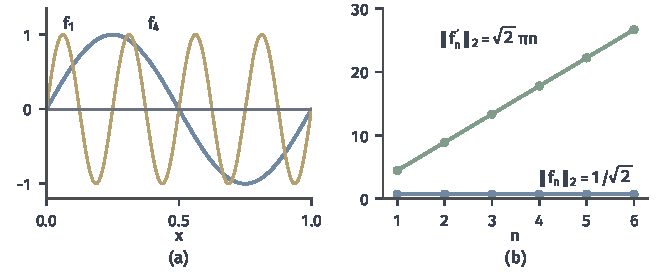
\includegraphics[width=112mm]{figures/04-spaces-measures-and-geometry/03-function-spaces/matplotlib/sobolev-oscillation/figure.pdf}
  \caption{振荡在$L^2$范数中不可见。(a)蓝色为$f_1$，黄色为$f_4$，其中$f_n(x)=\sin(2\pi nx)$，两者的$L^2$长度都是$1/\sqrt2$。(b)蓝点为$\lVert f_n\rVert_2$，保持不变；绿点为$\lVert f_n'\rVert_2$，按式~\eqref{eq:sobolev-oscillation-derivative}随$n$线性增长。}
  \label{fig:sobolev-oscillation}
\end{BookInlineFigure}

\paragraph{高频坐标上的权重}
用向量的语言重述这个现象。把$\sqrt2\sin(2\pi nx)$看成$L^2(0,1)$中的单位向量，它们两两正交，$f_n$就是沿第$n$条坐标轴、长度为$1/\sqrt2$的向量。求导把这条轴送到余弦轴上，同时把长度乘以$2\pi n$。所以频率越高的坐标，求导后放大得越多。

若把长度的平方改成“函数的平方加导数的平方”，第$n$条轴上的贡献就变成
\[
\lVert f_n\rVert_2^2+\lVert f_n'\rVert_2^2
=\frac12\bigl(1+(2\pi n)^2\bigr).
\]
这里的$1+(2\pi n)^2$就是一个权，高频坐标的权大，低频坐标的权小。把导数放进范数，相当于把各向同性的球压扁成沿高频方向很短的椭球。

有限维里可以把这件事完整算出来。取三个等距点上的取值$u=(u_1,u_2,u_3)$，用相邻差分$Du=(u_2-u_1,\ u_3-u_2)$代替导数。差分的平方和是一个二次型：
\[
\lVert Du\rVert^2=u^\top D^\top Du,\qquad
D^\top D=\begin{bmatrix}1&-1&0\\-1&2&-1\\0&-1&1\end{bmatrix}.
\]

这个矩阵的三个特征向量正好是三种“形状”，下面逐个验证。常向量$c=(1,1,1)$的相邻差为零，$D^\top Dc=0$，特征值是$0$。斜坡$t=(1,0,-1)$满足$D^\top Dt=t$，特征值是$1$。锯齿$z=(1,-2,1)$满足
\[
D^\top Dz=(3,-6,3)=3z,
\]
特征值是$3$。形状越“抖”，特征值越大。

于是在这组正交方向上，$\lVert u\rVert^2+\lVert Du\rVert^2$就是把三个坐标分别乘以权$1,2,4$再求和。以$z$为例：
\[
\lVert z\rVert^2=6,\qquad Dz=(-3,3),\qquad \lVert Dz\rVert^2=18=3\lVert z\rVert^2.
\]
函数空间的情形是同一幅图，只是坐标有无穷多个，权也趋于无穷。有限维时权总是有界的；无限维时权无界，这就是求导在$L^2$上不是有界算子的原因。

\paragraph{常数方向}
上面的权里常向量对应的导数项是零，这一点在函数上同样成立。常数函数$c$的导数为零，$\lVert c'\rVert_2=0$对每个$c$成立，只看导数无法区分$c=0$和$c=100$。导数度量变化，函数处在什么高度要由函数本身的大小记录。

所以完整的度量必须同时保留$\lVert f\rVert_2$和$\lVert f'\rVert_2$，也就是上面权里的“$1$”。只有附加零边界或零均值条件、排除了常数方向以后，导数才可能单独控制函数，这是第~\ref{sec:sobolev-derivative-norms}小节的问题。

\subsection{折点与跳跃}
\label{sec:sobolev-kinks-jumps}

若坚持经典导数，$f(x)=|x-1/2|$就会被排除：它只在$x=1/2$处没有导数，其余各点都光滑，变化速度恒为$1$。可是从“累积变化量”的角度看，这个函数没有任何异常。我们用第~\ref{chap:smoothing-weak-derivatives}章的弱导数来检查它。

令$g(x)=\operatorname{sgn}(x-1/2)$，即$x<1/2$时取$-1$，$x>1/2$时取$1$。任取测试函数$\varphi\in C_c^\infty(0,1)$，在折点两侧分别分部积分：
\[
\begin{aligned}
\int_0^1 f\varphi'\,\mathrm dx
&=\int_0^{1/2}\Bigl(\frac12-x\Bigr)\varphi'\,\mathrm dx
+\int_{1/2}^1\Bigl(x-\frac12\Bigr)\varphi'\,\mathrm dx\\
&=\int_0^{1/2}\varphi\,\mathrm dx-\int_{1/2}^1\varphi\,\mathrm dx
=-\int_0^1 g\varphi\,\mathrm dx .
\end{aligned}
\]
边界项在$x=1/2$处都含因子$f(1/2)=0$，在端点处$\varphi$为零，所以全部消失。按弱导数的定义，$f'=g$。

折点函数和它的弱导数都平方可积，大小可以直接算出：
\[
\lVert f\rVert_2^2=2\int_0^{1/2}t^2\,\mathrm dt=\frac1{12},\qquad
\lVert f'\rVert_2^2=1 .
\]
单点不能经典求导并不妨碍用$\lVert f\rVert_2$和$\lVert f'\rVert_2$同时控制它。把这类函数放在一起，就得到第~\ref{sec:sobolev-norms-completeness}节将记为$H^1(0,1)$的空间。

阶跃函数的情形不同。令$H=\mathbf 1_{[1/2,1)}$，对测试函数$\varphi$计算
\begin{equation}
-\int_0^1 H\varphi'\,\mathrm dx=-\int_{1/2}^1\varphi'\,\mathrm dx=\varphi(1/2).
\label{eq:sobolev-step-action}
\end{equation}
跳跃把测试函数送到它在跳跃点的取值，图~\ref{fig:sobolev-kink-step}的(d)画的就是这一作用。

\begin{BookInlineFigure}
  \centering
  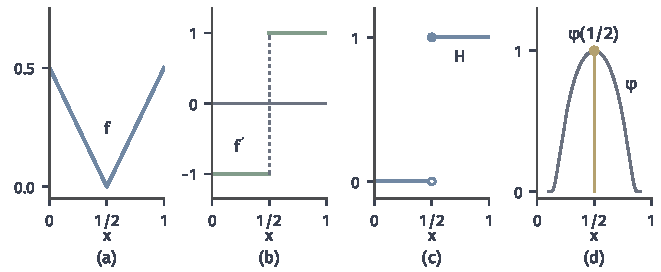
\includegraphics[width=112mm]{figures/04-spaces-measures-and-geometry/03-function-spaces/matplotlib/sobolev-kink-step/figure.pdf}
  \caption{折点与跳跃。(a)折点函数$f(x)=|x-1/2|$，连续。(b)它的弱导数$f'$，在$x=1/2$处跳跃，但仍是平方可积的函数。(c)阶跃函数$H$，在$x=1/2$处跳跃。(d)$H$对测试函数$\varphi$的作用只读取$\varphi(1/2)$，黄色竖线所示；这一作用集中在一点，不是任何函数的积分。}
  \label{fig:sobolev-kink-step}
\end{BookInlineFigure}

这个作用不能写成函数的积分。假设有局部可积函数$h$使$\int_0^1h\varphi\,\mathrm dx=\varphi(1/2)$对所有测试函数成立。对支撑不含$1/2$的$\varphi$，右端是零，由测试函数判别，$h$在$(0,1/2)$和$(1/2,1)$上都几乎处处为零。于是$h=0$几乎处处，而这与取$\varphi(1/2)\neq0$的测试函数矛盾。所以$H$没有弱导数，不属于上述空间。

阶跃函数在$x\neq1/2$处的经典导数是零，所以几乎处处导数是$0$。但$0$并不是它的弱导数，否则$H$几乎处处为常数。这个例子提醒我们，Sobolev空间中的“导数”始终指弱导数，几乎处处存在的经典导数不能自动代替它。

\paragraph{用余弦坐标比较}
现在把这些例子放到同一组坐标里。在$L^2(0,1)$上取正交归一基
\begin{equation}
e_0(x)=1,\qquad e_n(x)=\sqrt2\cos(\pi nx)\quad(n\geq1).
\label{eq:sobolev-cosine-basis}
\end{equation}
它是把函数偶延拓到$(-1,1)$后的Fourier基，完备性来自第~\ref{chap:fourier-transform}章。函数$f$的坐标是$a_n=\int_0^1fe_n\,\mathrm dx$，Parseval等式给出$\lVert f\rVert_2^2=\sum_na_n^2$。选用余弦基的原因在第~\ref{sec:sobolev-hk}小节说明。

先算折点函数的坐标。$f$关于$x=1/2$对称，而$n$为奇数时$\cos(\pi nx)$关于$x=1/2$反对称，所以奇数项为零。取$n=2m$，分部积分得
\[
\int_0^{1/2}\Bigl(\frac12-x\Bigr)\cos(2\pi mx)\,\mathrm dx
=\frac{1-\cos(\pi m)}{(2\pi m)^2}.
\]
因此$a_0=1/4$，而$n=2m$时
\[
a_{2m}=\frac{\sqrt2}{\pi^2m^2}\quad(m\text{为奇数}),\qquad
a_{2m}=0\quad(m\text{为偶数}).
\]

再算阶跃函数的坐标。$a_0=1/2$，$n\geq1$时直接积分得
\[
a_n=\sqrt2\int_{1/2}^1\cos(\pi nx)\,\mathrm dx
=-\frac{\sqrt2\,\sin(\pi n/2)}{\pi n}.
\]
所以偶数项为零，奇数项的绝对值是$\sqrt2/(\pi n)$。折点的坐标按$1/n^2$衰减，阶跃的坐标只按$1/n$衰减。

把坐标乘上权$\pi^2n^2$后求部分和，令$S_N=\sum_{n\leq N}\pi^2n^2a_n^2$。折点函数只有$n=2m$（$m$为奇数）的项，每项是
\[
\pi^2(2m)^2\cdot\frac{2}{\pi^4m^4}=\frac{8}{\pi^2m^2},
\]
再用$\sum_{m\text{奇}}m^{-2}=\pi^2/8$，得到$S_N\to1$，恰好等于$\lVert f'\rVert_2^2$。

阶跃函数的每个奇数项都是
\[
\pi^2n^2\cdot\frac{2}{\pi^2n^2}=2,
\]
所以$S_N$随$N$线性增长，趋于无穷。图~\ref{fig:sobolev-cosine-coordinates}对比了这两条路径：折点函数的加权和收敛到$1$，阶跃函数的加权和发散。

\begin{BookInlineFigure}
  \centering
  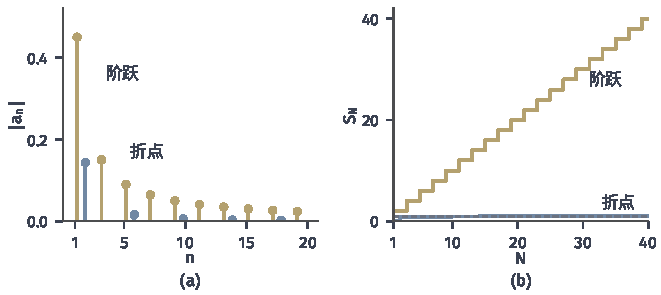
\includegraphics[width=112mm]{figures/04-spaces-measures-and-geometry/03-function-spaces/matplotlib/sobolev-cosine-coordinates/figure.pdf}
  \caption{折点与阶跃的余弦坐标。蓝色为折点函数$|x-1/2|$，黄色为阶跃函数$\mathbf 1_{[1/2,1)}$。(a)坐标的绝对值$|a_n|$，$n\geq1$。(b)加权部分和$S_N=\sum_{n\leq N}\pi^2n^2a_n^2$，虚线高度为$1$，折点的部分和收敛到这一高度，阶跃的部分和线性增长。}
  \label{fig:sobolev-cosine-coordinates}
\end{BookInlineFigure}

这就是用坐标看到的结论：Sobolev范数有限，等于坐标在加权后仍然平方可和。至于阶跃这样的跳跃应当怎样按尺度度量，第~\ref{chap:besov-spaces}章会用平移差回答。

\section{Sobolev范数与完备性}
\label{sec:sobolev-norms-completeness}

上一节的例子要求把函数与它的弱导数放在一起度量。本节固定三项数据，即区域$\Omega$、导数的最高阶数$k$和积分指数$p$，用$L^p$范数分别度量函数及各阶弱导数，再合成一个范数。然后证明这样得到的空间完备，并在$p=2$时写出它的内积和坐标形式。

\subsection{空间的定义}
\label{sec:sobolev-space-definition}

先约定记号。在欧氏开集$\Omega\subset\mathbb R^d$上，多重指标$\alpha=(\alpha_1,\ldots,\alpha_d)$由非负整数组成，$|\alpha|=\alpha_1+\cdots+\alpha_d$是导数的总阶数。$\partial^\alpha f$表示第~\ref{chap:smoothing-weak-derivatives}章意义下的弱导数，约定$\partial^0f=f$。

要询问$L^p$函数是否有弱导数，先要知道它局部可积。对紧集$K\subset\Omega$和$p<\infty$，Hölder不等式给出
\[
\int_K|f|\,\mathrm dx\leq|K|^{1-1/p}\lVert f\rVert_p,
\]
$p=\infty$时则有$\int_K|f|\leq|K|\,\lVert f\rVert_\infty$。所以$L^p$函数都局部可积，检验弱导数总是有意义的。

函数与每个导数各占一项，用下面的范数合在一起。

\begin{definition}[Sobolev空间]
\label{def:sobolev-space}
设$\Omega\subset\mathbb R^d$为开集，$k\geq0$为整数，$1\leq p\leq\infty$。所有满足下述条件的$f\in L^p(\Omega)$组成的集合记作$W^{k,p}(\Omega)$：对每个$|\alpha|\leq k$，弱导数$\partial^\alpha f$存在且属于$L^p(\Omega)$。称它为\term{Sobolev空间}（Sobolev space），并赋以\term{Sobolev范数}（Sobolev norm）
\begin{equation}
\lVert f\rVert_{W^{k,p}(\Omega)}=
\begin{cases}
\Bigl(\sum\limits_{|\alpha|\leq k}\lVert\partial^\alpha f\rVert_{L^p(\Omega)}^p\Bigr)^{1/p}, & 1\leq p<\infty,\\
\max\limits_{|\alpha|\leq k}\lVert\partial^\alpha f\rVert_{L^\infty(\Omega)}, & p=\infty .
\end{cases}
\label{eq:sobolev-norm}
\end{equation}
\end{definition}

三项数据各有分工。阶数$k$规定控制到第几阶导数，指数$p$规定函数和每个导数用哪种积分方式度量大小，区域$\Omega$规定在哪里检验测试恒等式。$k=0$时没有导数要求，$W^{0,p}(\Omega)=L^p(\Omega)$。区域不致混淆时，把$\lVert\cdot\rVert_{L^p(\Omega)}$简写为$\lVert\cdot\rVert_p$。

式~\eqref{eq:sobolev-norm}确实是范数。齐次性直接成立。三角不等式分两步：先对每个分量用$L^p$的Minkowski不等式，得到
\[
\lVert\partial^\alpha(f+g)\rVert_p\leq\lVert\partial^\alpha f\rVert_p+\lVert\partial^\alpha g\rVert_p,
\]
再把各分量的范数排成一个有限维向量，用$\ell^p$的Minkowski不等式合并。若范数为零，则零阶项$\lVert f\rVert_p=0$，$f$是零等价类。

把每个导数都计入范数，作用是让求导成为连续线性映射。对$|\alpha|\leq k$，把$\partial^\alpha$看成从$W^{k,p}(\Omega)$到$L^p(\Omega)$的映射，直接得到
\begin{equation}
\lVert\partial^\alpha f-\partial^\alpha g\rVert_p\leq\lVert f-g\rVert_{W^{k,p}} .
\label{eq:sobolev-derivative-continuous}
\end{equation}
这并不说明求导在$L^p$上连续：第~\ref{sec:sobolev-oscillation}小节的$f_n$在$L^2$中大小不变，导数却无界。连续性来自定义域的选择，导数的大小已经预先计入了输入的范数。

这里可以再用一次向量的类比。把$f$对应到有限个分量组成的“长向量”$(\partial^\alpha f)_{|\alpha|\leq k}$，它是乘积空间$L^p\times\cdots\times L^p$中的点，Sobolev范数就是这个长向量的范数。不同的是，这些分量并不独立：它们必须是同一个函数的各阶导数，受测试恒等式约束。Sobolev空间是乘积空间中满足这组约束的子集。

空间的元素是几乎处处等价类，弱导数也只确定到几乎处处。选不同的代表不改变元素，也不改变它的弱导数，但“某一点的函数值”一般没有意义，后面讨论端点值和边界值时必须专门处理。判断$f\in W^{k,p}(\Omega)$时，须对测试函数核对积分恒等式，不能用几乎处处的经典导数代替。

\begin{example}[折点函数的Sobolev范数]
\label{ex:sobolev-kink-norm}
在$(0,1)$上，$f(x)=|x-1/2|$的弱导数是$\operatorname{sgn}(x-1/2)$，二者都有界，所以$f\in W^{1,p}(0,1)$对每个$1\leq p\leq\infty$成立。

$p=2$时，由第~\ref{sec:sobolev-kinks-jumps}小节的计算，
\[
\lVert f\rVert_{W^{1,2}}^2=\frac1{12}+1=\frac{13}{12}.
\]
$p=\infty$时，两项的上确界分别是$1/2$和$1$，所以
\[
\lVert f\rVert_{W^{1,\infty}}=\max\Bigl(\frac12,\,1\Bigr)=1.
\]

$f$不属于$W^{2,p}(0,1)$。若二阶弱导数$h$存在，则$h$是$\operatorname{sgn}(x-1/2)$的弱导数。而
\[
\operatorname{sgn}(x-1/2)=2\,\mathbf 1_{[1/2,1)}(x)-1\quad\text{（几乎处处）},
\]
所以$h/2$是阶跃函数$H$的弱导数，这与上一节的结论矛盾。
\end{example}

\subsection{完备性}
\label{sec:sobolev-completeness}

$L^p(\Omega)$的完备性已在第~\ref{chap:function-normed-spaces}章证明，所以长向量$(\partial^\alpha f)_\alpha$的每个分量都有极限。需要说明的是，取极限以后各分量之间的约束仍然成立，也就是极限点仍在这个子集中。在乘积空间的图景里，这就是说该子集是闭的。

\begin{theorem}[Sobolev空间的完备性]
\label{thm:sobolev-complete}
设$\Omega\subset\mathbb R^d$为开集，$k\geq0$为整数，$1\leq p\leq\infty$。则$W^{k,p}(\Omega)$是Banach空间。
\end{theorem}

\begin{proof}
设$(f_n)$是$W^{k,p}(\Omega)$中的Cauchy列。

\emph{各分量的极限。}由式~\eqref{eq:sobolev-derivative-continuous}，对每个$|\alpha|\leq k$，$(\partial^\alpha f_n)_n$都是$L^p(\Omega)$中的Cauchy列。由$L^p$的完备性，存在$g_\alpha\in L^p(\Omega)$，使
\[
\partial^\alpha f_n\to g_\alpha\quad\text{在 }L^p(\Omega)\text{ 中}.
\]
记$f=g_0$。此时还不知道$g_\alpha$与$f$有什么关系，它们只是分别得到的极限。

\emph{把测试恒等式传到极限。}固定$\varphi\in C_c^\infty(\Omega)$，对每个$n$有
\[
\int_\Omega\partial^\alpha f_n\,\varphi\,\mathrm dx=(-1)^{|\alpha|}\int_\Omega f_n\,\partial^\alpha\varphi\,\mathrm dx .
\]
设$p'$为$p$的共轭指数。$\varphi$与$\partial^\alpha\varphi$有界且支撑紧，所以都属于$L^{p'}(\Omega)$。由Hölder不等式，
\[
\begin{aligned}
\Bigl|\int_\Omega(\partial^\alpha f_n-g_\alpha)\varphi\,\mathrm dx\Bigr|
&\leq\lVert\partial^\alpha f_n-g_\alpha\rVert_p\lVert\varphi\rVert_{p'},\\
\Bigl|\int_\Omega(f_n-f)\partial^\alpha\varphi\,\mathrm dx\Bigr|
&\leq\lVert f_n-f\rVert_p\lVert\partial^\alpha\varphi\rVert_{p'}.
\end{aligned}
\]
两式右端都趋于零。令$n\to\infty$，得到
\[
\int_\Omega g_\alpha\varphi\,\mathrm dx=(-1)^{|\alpha|}\int_\Omega f\,\partial^\alpha\varphi\,\mathrm dx
\]
对所有测试函数成立，即$g_\alpha=\partial^\alpha f$。

\emph{合并分量。}所有$\partial^\alpha f=g_\alpha$都属于$L^p(\Omega)$，所以$f\in W^{k,p}(\Omega)$。$p<\infty$时，
\[
\lVert f_n-f\rVert_{W^{k,p}}^p=\sum_{|\alpha|\leq k}\lVert\partial^\alpha f_n-g_\alpha\rVert_p^p\to0;
\]
$p=\infty$时把有限和换成有限个量的最大值，结论相同。
\end{proof}

证明的关键在第二步：测试恒等式两边都是对$L^p$收敛连续的线性量，所以约束在极限下保持。证明没有用到区域边界的形状，也没有得到逐点收敛或边界值，这些问题后面另行处理。

\subsection{\texorpdfstring{$H^k$}{Hk}空间}
\label{sec:sobolev-hk}

$p=2$时，函数与各阶导数都用平方积分度量，这些平方积分可以由内积给出。记$H^k(\Omega)=W^{k,2}(\Omega)$，定义
\begin{equation}
\langle f,g\rangle_{H^k}=\sum_{|\alpha|\leq k}\int_\Omega\partial^\alpha f\,\partial^\alpha g\,\mathrm dx .
\label{eq:sobolev-hk-inner}
\end{equation}

每一项都是$L^2(\Omega)$的内积，所以式~\eqref{eq:sobolev-hk-inner}有限，对两个变量都线性，并且对称。$f$与自身的内积正是Sobolev范数的平方，零阶项保证它只在$f=0$时为零。$k=1$时，
\[
\langle f,g\rangle_{H^1}=\int_\Omega fg\,\mathrm dx+\int_\Omega\nabla f\cdot\nabla g\,\mathrm dx .
\]

有限个$L^2$内积相加得到的只是内积空间。称它为Hilbert空间，依靠的是定理~\ref{thm:sobolev-complete}的完备性。有了Hilbert结构，第~\ref{chap:function-inner-product-spaces}章的正交投影就可以用于$H^k(\Omega)$的闭子空间，例如第~\ref{sec:sobolev-constrained-subspaces}节的零边界子空间。

\paragraph{一维$H^1$的加权坐标}
现在把“加权范数”的说法落实为定理。在区间$(0,1)$上，取式~\eqref{eq:sobolev-cosine-basis}的余弦基，并取另一组正交归一基$s_n(x)=\sqrt2\sin(\pi nx)$，$n\geq1$。两组基用求导互相联系：$e_n'=-\pi n\,s_n$。下面的定理说，$H^1(0,1)$恰好是坐标列的一个加权$\ell^2$空间。

\begin{theorem}[$H^1(0,1)$的余弦坐标]
\label{thm:sobolev-cosine-coordinates}
设$f\in L^2(0,1)$的余弦坐标为$a_n=\int_0^1fe_n\,\mathrm dx$。则$f\in H^1(0,1)$当且仅当$\sum_{n\geq0}\pi^2n^2a_n^2<\infty$，并且此时
\begin{equation}
\lVert f\rVert_{H^1}^2=\sum_{n\geq0}(1+\pi^2n^2)\,a_n^2 .
\label{eq:sobolev-cosine-norm}
\end{equation}
\end{theorem}

\begin{proof}
先设$f\in H^1(0,1)$，并取它的绝对连续代表（第~\ref{chap:smoothing-weak-derivatives}章）。乘积$fs_n$绝对连续，几乎处处有$(fs_n)'=f's_n+fs_n'$，而$s_n'=\pi n\,e_n$。在$[0,1]$上积分：
\[
\int_0^1f's_n\,\mathrm dx+\pi n\int_0^1fe_n\,\mathrm dx
=\bigl[fs_n\bigr]_0^1=0 .
\]
边界项为零，是因为$s_n(0)=s_n(1)=0$。所以$f'$的正弦坐标是$-\pi n\,a_n$。对$f'$用正弦基的Parseval等式，得到
\[
\lVert f'\rVert_2^2=\sum_{n\geq1}\pi^2n^2a_n^2 .
\]

反过来，设加权和有限。令部分和$F_N=\sum_{n\leq N}a_ne_n$，它是光滑函数，$F_N'=-\sum_{n\leq N}\pi n\,a_n\,s_n$。对$M<N$，
\[
\lVert F_N-F_M\rVert_{H^1}^2=\sum_{M<n\leq N}(1+\pi^2n^2)\,a_n^2\to0,
\]
所以$(F_N)$是$H^1(0,1)$中的Cauchy列。由定理~\ref{thm:sobolev-complete}它有极限，而$F_N\to f$在$L^2$中成立，所以极限就是$f$，$f\in H^1(0,1)$。式~\eqref{eq:sobolev-cosine-norm}由两次Parseval等式相加得到。
\end{proof}

余弦基的好处在证明里看得很清楚：分部积分的边界项被$s_n$在端点的零值消掉，所以定理对$H^1(0,1)$的每个函数都成立，不需要边界条件。可以用$f(x)=x$核对。分部积分得$a_n=\sqrt2((-1)^n-1)/(\pi^2n^2)$，只有奇数项非零，权重后的每项是$8/(\pi^2n^2)$，于是
\[
\sum_{n\text{奇}}\pi^2n^2a_n^2=\frac8{\pi^2}\cdot\frac{\pi^2}8=1=\lVert f'\rVert_2^2.
\]

把类比的对应关系和失效之处列在表~\ref{tab:sobolev-weight-analogy}中。最重要的是后两行：加权坐标只是$p=2$、$k=1$时最干净的图景，它帮助理解机制，但不能替代后面对一般$p$和一般区域的证明。

\begin{BookInlineTable}
  \centering
  \caption{有限维二次型与$H^1(0,1)$的对应。}
  \label{tab:sobolev-weight-analogy}
  \begin{tabular}{lll}
    \toprule
    & 三点差分 & $H^1(0,1)$\\
    \midrule
    坐标方向 & 常向量、斜坡、锯齿 & $e_0,e_1,e_2,\ldots$\\
    权 & $1,2,4$，有界 & $1+\pi^2n^2$，无界\\
    零导数方向 & 常向量 & 常数$e_0$\\
    $k\geq2$ & 权换成$D^\top D$的幂 & 需要边界相容条件\\
    $p\neq2$ & 没有正交坐标 & 没有正交坐标\\
    \bottomrule
  \end{tabular}
\end{BookInlineTable}

表中$k\geq2$一行需要解释。权$n^4$不再描述整个$H^2(0,1)$：$f(x)=x$属于$H^2(0,1)$，它的坐标却满足$n^4a_n^2\to$正常数（沿奇数$n$），加权和发散。分部积分此时要把一次导数的边界值也消掉，余弦坐标只描述满足$f'(0)=f'(1)=0$的子空间。周期函数没有这个问题，第~\ref{sec:sobolev-continuous-representatives}小节末尾还会用到周期情形。

\section{光滑函数的稠密性}
\label{sec:sobolev-smooth-density}

Sobolev函数可以有折点，也可以无界，直接对它们做计算往往不方便。常用的办法是先对光滑函数证明某个等式或估计，再用光滑函数逼近一般的Sobolev函数，让结论在极限中保留下来。这要求光滑函数在Sobolev范数下稠密：不仅函数本身要接近，每个弱导数分量也要同时接近。本节对任意开集和有限指数证明这一点，所用工具是第~\ref{chap:smoothing-weak-derivatives}章的磨光与第~\ref{chap:function-approximation}章的$L^p$磨光收敛。

\paragraph{需要的两条磨光结论}
记$\rho_\varepsilon(x)=\varepsilon^{-d}\rho(x/\varepsilon)$为第~\ref{chap:smoothing-weak-derivatives}章的磨光核：$\rho\geq0$光滑，支撑在单位闭球内，积分为$1$。对局部可积的$f$，记$\Omega_\varepsilon=\{x\in\Omega:\operatorname{dist}(x,\partial\Omega)>\varepsilon\}$，磨光$f_\varepsilon=f*\rho_\varepsilon$在$\Omega_\varepsilon$上光滑。若$f$有局部可积的弱导数$\partial^\alpha f$，则在$\Omega_\varepsilon$上
\begin{equation}
\partial^\alpha(f*\rho_\varepsilon)=(\partial^\alpha f)*\rho_\varepsilon ,
\label{eq:sobolev-mollifier-commute}
\end{equation}
左端是光滑函数的经典导数，右端是弱导数的磨光。这是第~\ref{chap:smoothing-weak-derivatives}章的结论。另一条结论来自第~\ref{chap:function-approximation}章：在全空间上，对$1\leq p<\infty$和$g\in L^p(\mathbb R^d)$，有$\lVert g*\rho_\varepsilon-g\rVert_p\to0$。

把两条结论用于$\Omega=\mathbb R^d$上的$f\in W^{k,p}(\mathbb R^d)$，此时$\Omega_\varepsilon=\mathbb R^d$。对每个$|\alpha|\leq k$，式\eqref{eq:sobolev-mollifier-commute}给出$\partial^\alpha f_\varepsilon-\partial^\alpha f=(\partial^\alpha f)*\rho_\varepsilon-\partial^\alpha f$，它在$L^p$中趋于零。有限多个分量都趋于零，所以
\begin{equation}
\lVert f*\rho_\varepsilon-f\rVert_{W^{k,p}(\mathbb R^d)}\to0\qquad(\varepsilon\to0,\ 1\leq p<\infty).
\label{eq:sobolev-whole-space-mollify}
\end{equation}
在一般开集上，磨光只在$\Omega_\varepsilon$上有定义，越靠近边界，允许的磨光半径越小。解决办法是把函数切成许多块，每块离边界的距离不同，各自选择磨光半径，再拼回去。切块需要光滑的截断函数与乘积法则。

\paragraph{截断函数}
先构造在给定紧集上取值为$1$、支撑仍在指定开集内的光滑函数。

\begin{lemma}[截断函数]
\label{lem:sobolev-cutoff}
设$K\subset V\subset\mathbb R^d$，$K$紧，$V$开。则存在$\eta\in C_c^\infty(V)$，使$0\leq\eta\leq1$，并且在$K$上$\eta=1$。
\end{lemma}

\begin{proof}
$V=\mathbb R^d$时取$\delta=1$；否则$K$到闭集$\mathbb R^d\setminus V$的距离为正，取$\delta$为这个距离的四分之一。令$U=\{x:\operatorname{dist}(x,K)<2\delta\}$，$\eta=\mathbf 1_U*\rho_\delta$。由磨光的光滑性，$\eta$光滑；由$\rho_\delta\geq0$且积分为$1$，$0\leq\eta\leq1$。若$x\in K$，球$B(x,\delta)\subset U$，于是$\eta(x)=\int_{B(x,\delta)}\rho_\delta(x-y)\,\mathrm dy=1$。若$\operatorname{dist}(x,K)>3\delta$，球$B(x,\delta)$与$U$不交，$\eta(x)=0$。所以$\eta$的支撑含于紧集$\{x:\operatorname{dist}(x,K)\leq3\delta\}\subset V$。
\end{proof}

称这样的$\eta$为\term{截断函数}（cutoff function）。用它乘一个函数，可以把函数限制在指定区域附近，而不引入不光滑的边缘。

\paragraph{乘积法则}
截断后的函数是否仍在Sobolev空间中，取决于光滑函数与Sobolev函数的乘积怎样求弱导数。

\begin{lemma}[光滑函数的乘积法则]
\label{lem:sobolev-product-rule}
设$f\in W^{k,p}(\Omega)$，$\zeta\in C^\infty(\Omega)$且$\zeta$及其各阶导数在$\Omega$上有界。则$\zeta f\in W^{k,p}(\Omega)$，一阶弱导数为$\partial_i(\zeta f)=\zeta\,\partial_if+(\partial_i\zeta)f$，并且存在只依赖$k,d$与$\zeta$的各阶导数上界的常数$C$，使$\lVert\zeta f\rVert_{W^{k,p}}\leq C\lVert f\rVert_{W^{k,p}}$。
\end{lemma}

\begin{proof}
对测试函数$\varphi$，$\zeta\varphi$仍是测试函数，经典乘积法则给出$\zeta\,\partial_i\varphi=\partial_i(\zeta\varphi)-(\partial_i\zeta)\varphi$。于是
\begin{equation*}
\begin{aligned}
\int_\Omega\zeta f\,\partial_i\varphi\,\mathrm dx&=\int_\Omega f\,\partial_i(\zeta\varphi)\,\mathrm dx-\int_\Omega f(\partial_i\zeta)\varphi\,\mathrm dx\\
&=-\int_\Omega\bigl(\zeta\,\partial_if+(\partial_i\zeta)f\bigr)\varphi\,\mathrm dx ,
\end{aligned}
\end{equation*}
第二个等号对测试函数$\zeta\varphi$用了$f$的弱导数定义。右端括号内的函数属于$L^p$，范数不超过$\sup|\zeta|\,\lVert\partial_if\rVert_p+\sup|\partial_i\zeta|\,\lVert f\rVert_p$。高阶情形对阶数归纳：$\zeta\,\partial_if$与$(\partial_i\zeta)f$都是“有界光滑函数乘以$W^{k-1,p}$函数”，对它们再用一阶结论。每一步只出现$\zeta$的有限个导数与$f$的有限个弱导数，范数界由此得到。
\end{proof}

\paragraph{局部有限的单位分解}
现在把$\Omega$按离边界的远近分层。令
\[
G_j=\{x\in\Omega:|x|<j,\ \operatorname{dist}(x,\mathbb R^d\setminus\Omega)>1/j\},\qquad j\geq1,
\]
$\Omega=\mathbb R^d$时省去距离条件，并约定$G_0=G_{-1}=\varnothing$。每个$G_j$是开集，闭包是$\Omega$内的紧集，$\overline{G_j}\subset G_{j+1}$，并且$\bigcup_jG_j=\Omega$。令$V_j=G_{j+1}\setminus\overline{G_{j-1}}$。这些开集覆盖$\Omega$，并且是\term{局部有限}（locally finite）的：$G_m$只与$V_1,\ldots,V_{m+1}$相交，所以每点有一个邻域只碰到有限多个$V_j$。

由引理~\ref{lem:sobolev-cutoff}，对紧集$\overline{G_j}\setminus G_{j-1}\subset V_j$取截断函数$\eta_j\in C_c^\infty(V_j)$，在该紧集上$\eta_j=1$。这些紧集覆盖$\Omega$，所以$S=\sum_i\eta_i$处处至少为$1$；由局部有限性，它在每点附近只是有限和，因而光滑。令$\zeta_j=\eta_j/S$，则$\zeta_j\in C_c^\infty(V_j)$，$0\leq\zeta_j\leq1$，并且在$\Omega$上$\sum_j\zeta_j=1$，每点附近只有有限项非零。称$\{\zeta_j\}$为从属于覆盖$\{V_j\}$的\term{单位分解}（partition of unity）。

\begin{theorem}[开集内光滑函数的稠密性]
\label{thm:sobolev-meyers-serrin}
设$\Omega\subset\mathbb R^d$为任意开集，$k\geq0$为整数，$1\leq p<\infty$。则$C^\infty(\Omega)\cap W^{k,p}(\Omega)$在$W^{k,p}(\Omega)$中稠密。
\end{theorem}

\begin{proof}
固定$f\in W^{k,p}(\Omega)$与$\theta>0$。

\emph{分块。}令$f_j=\zeta_jf$。由引理~\ref{lem:sobolev-product-rule}，$f_j\in W^{k,p}(\Omega)$，且它和各阶弱导数都在$\operatorname{supp}\zeta_j\subset V_j$之外为零。把$f_j$在$\Omega$外补成零，得到的函数仍记为$f_j$，它属于$W^{k,p}(\mathbb R^d)$：对$\mathbb R^d$上的测试函数$\varphi$，取在$\operatorname{supp}\zeta_j$上为$1$、支撑在$\Omega$内的截断函数$\chi$，则$\int f_j\,\partial^\alpha\varphi=\int f_j\,\partial^\alpha(\chi\varphi)$，而$\chi\varphi$是$\Omega$上的测试函数，所以测试恒等式在全空间成立。

\emph{逐块磨光。}由式\eqref{eq:sobolev-whole-space-mollify}，可取$\varepsilon_j>0$，使$g_j=f_j*\rho_{\varepsilon_j}$满足
\[
\lVert g_j-f_j\rVert_{W^{k,p}(\mathbb R^d)}<\theta\,2^{-j}.
\]
$g_j$的支撑落在$\operatorname{supp}\zeta_j$的$\varepsilon_j$邻域内。$\operatorname{supp}\zeta_j$是$V_j$中的紧集，而$V_j\subset W_j:=G_{j+2}\setminus\overline{G_{j-2}}$且$\overline{V_j}$与$W_j$的补集有正距离，再缩小$\varepsilon_j$，可使$\operatorname{supp}g_j\subset W_j$。误差按$2^{-j}$分配，是为了让总和不超过$\theta$。

\emph{拼合。}令$g=\sum_jg_j$。每点有邻域只与有限多个$W_j$相交，所以$g$在这个邻域上是有限个光滑函数之和，$g\in C^\infty(\Omega)$。同样，在每个$G_m$上，$f=\sum_jf_j$也只是有限和。于是
\[
\lVert g-f\rVert_{W^{k,p}(G_m)}\leq\sum_j\lVert g_j-f_j\rVert_{W^{k,p}(\mathbb R^d)}<\theta .
\]
令$m\to\infty$，由单调收敛定理得$\lVert g-f\rVert_{W^{k,p}(\Omega)}\leq\theta$，特别地$g\in W^{k,p}(\Omega)$。
\end{proof}

这个定理对任意开集成立，不需要边界的任何正则性。但要读清它给出了什么：逼近函数只在$\Omega$内部光滑，在边界附近可以剧烈振荡；它们一般不是紧支撑的，也不一定能连续地延伸到边界。紧支撑光滑函数在$W^{k,p}(\Omega)$中一般并不稠密，第~\ref{sec:sobolev-endpoint-values}小节将看到，$(0,1)$上的常数$1$与所有紧支撑光滑函数的$H^1$距离至少为$1/\sqrt2$。若要求逼近函数光滑到边界，需要先把函数延拓到区域之外，这是下一节的任务。

指数条件$p<\infty$不能去掉。考虑$(0,1)$上的$f(x)=|x-1/2|$与任一$v\in C^1(0,1)\cap W^{1,\infty}(0,1)$。$v'$在$1/2$处连续，所以在$1/2$的足够小邻域内$|v'(x)-v'(1/2)|<\delta$；而$f'$在该点左侧为$-1$、右侧为$1$，因此
\[
\lVert v'-f'\rVert_\infty\geq\max\bigl(|v'(1/2)+1|,\,|v'(1/2)-1|\bigr)-\delta\geq1-\delta .
\]
$\delta$可以任意小，于是$\lVert v-f\rVert_{W^{1,\infty}}\geq1$：本质上确界范数要求导数在每个小邻域都一致接近，连续导数无法一致逼近跳跃的导数。

\section{跨边界延拓}
\label{sec:sobolev-extension}

许多论证希望在全空间$\mathbb R^d$上进行，那里磨光不受边界限制，平移和缩放也可以自由使用。为此要把区域$\Omega$上的Sobolev函数延拓成全空间上的Sobolev函数，并且延拓后的范数受原范数控制。这和把一段向量补长不同：补上去的部分不能破坏弱导数的存在。本节先在平直边界附近用反射说明函数怎样越过边界，再在有界Lipschitz区域上陈述一般的延拓定理，并由此得到光滑到边界的逼近。

\paragraph{一维反射}
设$f\in W^{1,p}(0,1)$，$1\leq p<\infty$。由第~\ref{chap:smoothing-weak-derivatives}章，$f$有绝对连续代表，仍记为$f$。在$(-1,1)$上令$Ef(x)=f(|x|)$。它在$[-1,0]$和$[0,1]$上分别绝对连续，并在$x=0$处取同一个值$f(0)$，所以在$[-1,1]$上绝对连续，几乎处处导数为$\operatorname{sgn}(x)f'(|x|)$。

绝对连续函数的几乎处处导数就是它的弱导数，因此$Ef\in W^{1,p}(-1,1)$。两侧对称，范数正好翻倍：
\begin{equation}
\lVert Ef\rVert_{W^{1,p}(-1,1)}^p=2\lVert f\rVert_{W^{1,p}(0,1)}^p .
\label{eq:sobolev-reflection-norm}
\end{equation}
用$f(x)=1+x-x^2$手算一次。$p=2$时，
\[
\int_0^1f^2\,\mathrm dx=\frac{41}{30},\qquad
\int_0^1(f')^2\,\mathrm dx=\int_0^1(1-2x)^2\,\mathrm dx=\frac13,
\]
所以$\lVert f\rVert_{H^1(0,1)}^2=17/10$，延拓后是$17/5$。

图~\ref{fig:sobolev-reflections}的(a)画的就是这个偶反射。反射在原点通常产生一个折点，正如$|x|$那样，但折点不破坏一阶弱导数的存在，因为两侧的值连在一起。

\begin{BookInlineFigure}
  \centering
  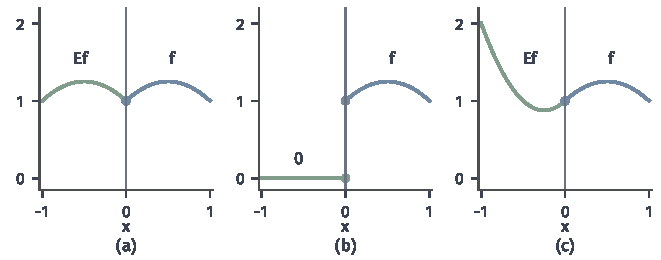
\includegraphics[width=112mm]{figures/04-spaces-measures-and-geometry/03-function-spaces/matplotlib/sobolev-reflections/figure.pdf}
  \caption{同一函数$f(x)=1+x-x^2$的三种延拓，蓝色为原函数，绿色为$x<0$一侧补上的部分。(a)偶反射，在原点连续，但有折点，属于$H^1$，一般不属于$H^2$。(b)零延拓，在原点跳跃，不属于$H^1$。(c)二阶反射$Ef(x)=-3f(-x)+4f(-x/2)$，在原点函数值和一阶导数都相接，属于$H^2$。}
  \label{fig:sobolev-reflections}
\end{BookInlineFigure}

\paragraph{半空间上的偶反射}
高维时最简单的边界是超平面。记$\mathbb R^d_+$为$x_d>0$的半空间，点写成$x=(x',x_d)$，其中$x'\in\mathbb R^{d-1}$。设$f$在闭半空间上连续可微、支撑有界，作偶反射
\[
Ef(x',x_d)=f(x',|x_d|).
\]
我们验证它在全空间有弱导数。对$i<d$，反射不涉及$x_i$，在两个半空间内分别分部积分，就得到$\partial_iEf(x',x_d)=(\partial_if)(x',|x_d|)$。

对$i=d$，取测试函数$\varphi\in C_c^\infty(\mathbb R^d)$，固定$x'$，分别在$x_d>0$和$x_d<0$上对$x_d$分部积分：
\[
\begin{aligned}
\int_0^\infty f(x',t)\,\partial_d\varphi\,\mathrm dt
&=-f(x',0)\varphi(x',0)-\int_0^\infty\partial_df\,\varphi\,\mathrm dt,\\
\int_{-\infty}^0 f(x',-t)\,\partial_d\varphi\,\mathrm dt
&=f(x',0)\varphi(x',0)+\int_{-\infty}^0(\partial_df)(x',-t)\,\varphi\,\mathrm dt .
\end{aligned}
\]
第二式用了链式法则：$t\mapsto f(x',-t)$的导数是$-(\partial_df)(x',-t)$。

两式相加，边界面上的项$\pm f(x',0)\varphi(x',0)$恰好相消。再对$x'$积分，得
\[
\int_{\mathbb R^d}Ef\,\partial_d\varphi\,\mathrm dx
=-\int_{\mathbb R^d}\operatorname{sgn}(x_d)\,(\partial_df)(x',|x_d|)\,\varphi\,\mathrm dx .
\]
所以
\[
\partial_dEf=\operatorname{sgn}(x_d)\,(\partial_df)(x',|x_d|).
\]
两侧对称，范数恒等式与式~\eqref{eq:sobolev-reflection-norm}相同：全空间上的$p$次方范数是半空间上的两倍。

上面的计算要求$f$光滑到边界并且支撑有界，一般的$f\in W^{1,p}(\mathbb R^d_+)$（$1\leq p<\infty$）可以这样逼近。先用$\chi(x/R)$截断，由引理~\ref{lem:sobolev-product-rule}和控制收敛，$R\to\infty$时误差趋于零。再向内部平移，$f_h(x',x_d)=f(x',x_d+h)$在更大的半空间$x_d>-h$上有定义，用半径小于$h$的磨光，就得到在闭半空间上光滑、支撑有界的函数。令$h$与磨光半径趋于零，由平移的积分连续性和磨光收敛，这些函数在$W^{1,p}(\mathbb R^d_+)$中趋于截断后的函数。

于是$E$在一个稠密子空间上满足上述范数恒等式。由$W^{1,p}(\mathbb R^d)$的完备性，它唯一地延伸为整个$W^{1,p}(\mathbb R^d_+)$上的有界线性算子，延伸后的$Ef$仍几乎处处等于$f(x',|x_d|)$。

\paragraph{零延拓与边界相容条件}
与偶反射对照，把$f$在$x_d<0$处直接补成零，称为\term{零延拓}（zero extension）。重做上面的分部积分，只剩$x_d>0$一侧，边界项
\[
-\int_{\mathbb R^{d-1}}f(x',0)\,\varphi(x',0)\,\mathrm dx'
\]
不再被抵消。若$f$在边界面上的值不恒为零，这一项集中在零测的超平面上，不能写成$\int g\varphi$的形式，论证与阶跃函数相同。图~\ref{fig:sobolev-reflections}的(b)是一维的情形：跳跃出现在接缝处，$(0,1)$上的常数$1$零延拓后就是阶跃函数，不属于$W^{1,p}(-1,1)$。

所以零延拓需要边界相容条件：函数在边界上的值为零。对光滑到边界的函数，这一条件可以逐点检查。对一般的Sobolev函数，“边界值”要通过第~\ref{sec:sobolev-trace}小节的迹来理解。第~\ref{sec:sobolev-compact-closure}小节的闭包空间恰好由这类函数组成，零延拓在其上保持范数不变。

\paragraph{高阶延拓}
偶反射对$W^{2,p}$不够。反射后$\partial_dEf$在$x_d>0$一侧趋于$\partial_df(x',0)$，在另一侧趋于$-\partial_df(x',0)$。只要法向导数在边界上不为零，$\partial_dEf$就有跳跃，没有局部可积的弱导数。高阶延拓必须让函数及其直到$k-1$阶的法向导数在边界两侧相接。

对$k=2$，可以在$x_d<0$处令
\begin{equation}
Ef(x',x_d)=-3f(x',-x_d)+4f\Bigl(x',-\frac{x_d}{2}\Bigr).
\label{eq:sobolev-second-order-reflection}
\end{equation}
系数的选取是为了让两个条件同时成立。在$x_d=0$处，函数值为$-3f+4f=f(x',0)$。对$x_d$求导，得到
\[
\partial_dEf(x',x_d)=3\,\partial_df(x',-x_d)-2\,\partial_df\Bigl(x',-\frac{x_d}2\Bigr),
\]
它在边界上等于$\partial_df(x',0)$。

用图~\ref{fig:sobolev-reflections}(c)的函数手算核对。$f(x)=1+x-x^2$代入式~\eqref{eq:sobolev-second-order-reflection}，$x<0$时得
\[
Ef(x)=-3(1-x-x^2)+4\Bigl(1-\frac x2-\frac{x^2}4\Bigr)=1+x+2x^2 .
\]
在$x=0$处函数值都是$1$，一阶导数都是$1$。二阶导数左侧是$4$，右侧是$-2$，有跳跃，但二阶导数只需要作为$L^p$函数存在。

一般地，$Ef$在全空间连续可微，两侧分别二阶光滑，按前面的分部积分，二阶弱导数存在且局部可积。$x_d<0$一侧的各阶导数是$f$的导数在两个缩放位置的有限组合，换元后得到
\[
\lVert Ef\rVert_{W^{2,p}(\mathbb R^d)}\leq C\lVert f\rVert_{W^{2,p}(\mathbb R^d_+)} .
\]
对一般的$k$，取$k$个系数使前$k$个法向导数都相接即可。

\paragraph{Lipschitz区域}
一般区域的边界可以弯曲，甚至有棱角。只要边界在每点附近都能写成函数图像，并且区域只位于图像的一侧，就可以在局部把边界拉直，再用反射。

\begin{definition}[Lipschitz区域]
\label{def:sobolev-lipschitz-domain}
称有界开集$\Omega\subset\mathbb R^d$为\term{Lipschitz区域}（Lipschitz domain），若对每个$x_0\in\partial\Omega$，存在$r>0$、经旋转与平移得到的坐标$(x',x_d)$以及Lipschitz函数$\gamma:\mathbb R^{d-1}\to\mathbb R$，使
\begin{equation}
\Omega\cap B(x_0,r)=\{x\in B(x_0,r):x_d>\gamma(x')\}.
\label{eq:sobolev-lipschitz-graph}
\end{equation}
\end{definition}

图~\ref{fig:sobolev-lipschitz-domains}对比了三种情形。球、立方体和有界凸开集都是Lipschitz区域；立方体在棱角处不光滑，但把坐标轴转过去，局部仍是Lipschitz图像。挖去一条线段的圆盘不是：割缝两侧都属于区域，区域不能只位于割缝的一侧。

\begin{BookInlineFigure}
  \centering
  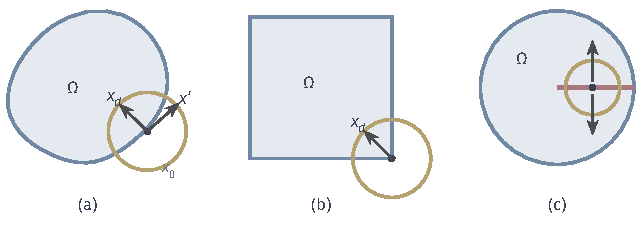
\includegraphics[width=108.356mm]{figures/04-spaces-measures-and-geometry/03-function-spaces/tikz/sobolev-lipschitz-domains/figure.pdf}
  \caption{Lipschitz区域的局部图像条件，黄圈为球$B(x_0,r)$。(a)弯曲边界，局部坐标中$x_d$指向区域内，$\Omega$位于图像$x_d=\gamma(x')$的上方。(b)方形的角点，把$x_d$轴转到对角线方向后，边界仍是Lipschitz图像。(c)割缝圆盘，红线为割缝，黄圈内区域同时位于割缝两侧，不能写成单侧图像，因而不是Lipschitz区域。}
  \label{fig:sobolev-lipschitz-domains}
\end{BookInlineFigure}

\begin{theorem}[Lipschitz区域上的延拓]
\label{thm:sobolev-extension}
设$\Omega\subset\mathbb R^d$为有界Lipschitz区域，$1\leq p<\infty$。存在有界线性算子$E:W^{1,p}(\Omega)\to W^{1,p}(\mathbb R^d)$和有界集合$B_\Omega$，使对每个$f\in W^{1,p}(\Omega)$，$Ef$在$\Omega$上几乎处处等于$f$，并且$Ef$在$B_\Omega$之外为零。
\end{theorem}

完整证明要处理Lipschitz变换下的弱导数，篇幅较长，读者可查阅Sobolev空间的专著，这里说明构造的步骤。边界是紧集，可以用有限个满足定义的球覆盖，再加上一个闭包含于$\Omega$的开集覆盖内部。取从属于这有限个开集的单位分解，把$f$分成有限块，内部那块在边界附近为零，直接零延拓。

每个边界块用变换$(x',x_d)\mapsto(x',x_d-\gamma(x'))$拉直为半空间上的函数，作偶反射，再变换回去。这个变换与它的逆都是Lipschitz映射，它们把$W^{1,p}$函数映为$W^{1,p}$函数，范数只相差由$\gamma$的Lipschitz常数决定的倍数。最后用一个固定的截断函数乘以和式，使所有延拓都在同一有界集合外为零。

这一构造对一阶空间有效，但不能直接推广到高阶：Lipschitz拉直变换只有一阶导数的控制，复合以后二阶导数一般不存在。若边界是$C^k$图像，可以用光滑的拉直变换配合上面的高阶反射。对一般有界Lipschitz区域，$W^{k,p}$的延拓也存在，但需要不同的构造，读者可查阅相关专著。

\paragraph{光滑到边界的逼近}
延拓定理的一个直接推论是更强的逼近：逼近函数可以取为全空间紧支撑光滑函数在$\Omega$上的限制，从而连同各阶导数都连续到边界。

\begin{theorem}[光滑到边界的逼近]
\label{thm:sobolev-smooth-up-to-boundary}
设$\Omega$为有界Lipschitz区域，$1\leq p<\infty$。则$\{\psi|_\Omega:\psi\in C_c^\infty(\mathbb R^d)\}$在$W^{1,p}(\Omega)$中稠密。
\end{theorem}

\begin{proof}
对$f\in W^{1,p}(\Omega)$，由定理~\ref{thm:sobolev-extension}得到在有界集合外为零的$Ef\in W^{1,p}(\mathbb R^d)$。$Ef*\rho_\varepsilon$光滑且支撑紧，由式~\eqref{eq:sobolev-whole-space-mollify}，它在$W^{1,p}(\mathbb R^d)$中趋于$Ef$。限制到$\Omega$上范数只会变小，所以
\[
\lVert(Ef*\rho_\varepsilon)|_\Omega-f\rVert_{W^{1,p}(\Omega)}
\leq\lVert Ef*\rho_\varepsilon-Ef\rVert_{W^{1,p}(\mathbb R^d)}\to0.
\qedhere
\]
\end{proof}

记这类限制函数的全体为$C^\infty(\overline\Omega)$。与定理~\ref{thm:sobolev-meyers-serrin}相比，这里多了边界正则性的假设，换来的是光滑到边界的逼近函数。下一节定义边界值时，正是先对这类函数直接限制到边界，再用逼近推广到整个空间。

\section{约束子空间}
\label{sec:sobolev-constrained-subspaces}

许多问题要求函数满足边界条件，例如在区间两端取零，或在区域边界上取指定的值。Sobolev函数是几乎处处等价类，而边界是零测集，任意修改边界上的值不改变元素，所以“边界值”不能取一个代表直接读出。本节先用紧支撑光滑函数的闭包定义零边界子空间，它不涉及任何边界值；再在一维用绝对连续代表读出端点值，在高维用迹映射表达边界值。最后研究零边界与零均值约束怎样排除常数方向，使导数单独给出等价范数。

\subsection{紧支撑光滑函数的闭包}
\label{sec:sobolev-compact-closure}

紧支撑光滑函数在边界附近恒为零。若一个Sobolev函数能被这样的函数在Sobolev范数下任意逼近，它就在极限意义上“在边界附近为零”。把这一想法直接取作定义。

\begin{definition}[零边界Sobolev空间]
\label{def:sobolev-w0}
设$\Omega\subset\mathbb R^d$为开集，$k\geq1$为整数，$1\leq p<\infty$。把$C_c^\infty(\Omega)$在$W^{k,p}(\Omega)$范数下的闭包记作$W_0^{k,p}(\Omega)$，称为\term{零边界Sobolev空间}（Sobolev space with zero boundary values），$p=2$时记作$H_0^k(\Omega)$。
\end{definition}

这里的闭包是第~\ref{chap:topological-spaces}章的概念：在由Sobolev范数给出的度量下，每个邻域都与$C_c^\infty(\Omega)$相交的元素全体。度量空间中，它恰好由$C_c^\infty(\Omega)$中序列的极限组成。若$\varphi_n\to f$、$\psi_n\to g$，则对实数$a,b$有$a\varphi_n+b\psi_n\to af+bg$，而$a\varphi_n+b\psi_n$仍是紧支撑光滑函数，所以闭包对线性组合封闭。闭包本身是闭集，于是$W_0^{k,p}(\Omega)$是$W^{k,p}(\Omega)$的闭线性子空间，由定理~\ref{thm:sobolev-complete}，它本身也是Banach空间。

定义只用到逼近，不需要区域边界的任何正则性。两个问题需要分别核对。第一，$W_0^{k,p}(\Omega)$一般是真子空间，下一小节将证明$(0,1)$上的常数$1$不属于$H_0^1(0,1)$。在全空间则没有边界：取在$|x|\leq1$上为$1$、在$|x|\geq2$外为零的截断函数$\chi$，$\chi(x/R)f$在$R\to\infty$时于$W^{k,p}(\mathbb R^d)$中趋于$f$，再对它磨光，可知$W_0^{k,p}(\mathbb R^d)=W^{k,p}(\mathbb R^d)$。第二，定义限于$p<\infty$。在$W^{1,\infty}$范数下，紧支撑光滑函数的极限具有一致连续的导数，第~\ref{sec:sobolev-smooth-density}节末尾的$|x-1/2|$与之距离至少为$1$；所以$p=\infty$时的闭包远小于“零边界的$W^{1,\infty}$函数”，有限指数的结论不能照搬。

\subsection{端点值}
\label{sec:sobolev-endpoint-values}

一维时，边界只有两个端点，而第~\ref{chap:smoothing-weak-derivatives}章已经证明$v\in H^1(0,1)$有绝对连续代表$\tilde v$，并且$\tilde v(y)-\tilde v(x)=\int_x^yv'(t)\,\mathrm dt$。端点值$\tilde v(0)$与$\tilde v(1)$由这个代表确定。我们需要知道它们是否受$H^1$范数控制。

把上式对$x\in(0,1)$积分。由于区间长度为$1$，
\[
\tilde v(y)=\int_0^1\tilde v(x)\,\mathrm dx+\int_0^1\int_x^yv'(t)\,\mathrm dt\,\mathrm dx,\qquad
|\tilde v(y)|\leq\int_0^1|v|\,\mathrm dx+\int_0^1|v'|\,\mathrm dt .
\]
再由Cauchy--Schwarz不等式，$\int_0^1|v|\leq\lVert v\rVert_2$，$\int_0^1|v'|\leq\lVert v'\rVert_2$。于是对每个$y\in[0,1]$，特别是两个端点，
\begin{equation}
|\tilde v(y)|\leq\lVert v\rVert_2+\lVert v'\rVert_2\leq\sqrt2\,\lVert v\rVert_{H^1(0,1)} .
\label{eq:sobolev-endpoint-bound}
\end{equation}
所以映射$v\mapsto\tilde v(0)$是线性的，并且对$H^1$范数连续；$v\mapsto\tilde v(1)$同理。式\eqref{eq:sobolev-endpoint-bound}还说明，$H^1$收敛蕴含连续代表的一致收敛。

只有$L^2$控制是不够的。$v_n(x)=\max(1-nx,0)$满足$v_n(0)=1$，而$\lVert v_n\rVert_2^2=\int_0^{1/n}(1-nx)^2\,\mathrm dx=1/(3n)\to0$。端点值能被控制，靠的是导数项：$\lVert v_n'\rVert_2=\sqrt n$随$n$增大。

现在把估计用于闭包。每个$\varphi\in C_c^\infty(0,1)$在端点为零。若$\varphi_n\to v$在$H^1$中成立，由式\eqref{eq:sobolev-endpoint-bound}，$\tilde v(0)=\lim\varphi_n(0)=0$，同理$\tilde v(1)=0$。所以$H_0^1(0,1)=W_0^{1,2}(0,1)$中的函数都有零端点值。常数$1$不满足这一条件，并且对每个$\varphi\in C_c^\infty(0,1)$，
\[
1=|1-\varphi(0)|\leq\sqrt2\,\lVert1-\varphi\rVert_{H^1},
\]
它到紧支撑光滑函数的$H^1$距离至少是$1/\sqrt2$。反过来，连续代表在两端为零的$H^1(0,1)$函数都属于$H_0^1(0,1)$，这是下一小节零迹刻画在一维的情形。

\subsection{迹映射}
\label{sec:sobolev-trace}

高维时，$W^{1,p}$函数一般没有连续代表，第~\ref{sec:sobolev-continuous-embeddings}节将给出在边界点附近无界的例子，因此不能逐点读取边界值。我们改为先对光滑到边界的函数直接限制到边界，证明限制的边界$L^p$大小受Sobolev范数控制，再用逼近推广。

\paragraph{半空间上的估计}
设$f\in C_c^1(\mathbb R^d)$，考虑它在闭半空间$\overline{\mathbb R^d_+}$上的部分。固定$x'$，沿$x_d$方向从边界点$(x',0)$向内积分。$t$足够大时$f(x',t)=0$，所以$p=1$时
\[
|f(x',0)|=\Bigl|\int_0^\infty\partial_df(x',t)\,\mathrm dt\Bigr|\leq\int_0^\infty|\partial_df(x',t)|\,\mathrm dt .
\]
$p>1$时$|f|^p$连续可微，导数的绝对值不超过$p|f|^{p-1}|\partial_df|$。由Young不等式$ab\leq a^{p'}/p'+b^p/p$（取$a=|f|^{p-1}$，$b=|\partial_df|$，$p'=p/(p-1)$），
\[
|f(x',0)|^p=-\int_0^\infty\partial_t\bigl(|f(x',t)|^p\bigr)\,\mathrm dt\leq\int_0^\infty\bigl((p-1)|f|^p+|\partial_df|^p\bigr)\,\mathrm dt .
\]
两种情形都对$x'\in\mathbb R^{d-1}$积分，得到
\begin{equation}
\int_{\mathbb R^{d-1}}|f(x',0)|^p\,\mathrm dx'\leq\max(p-1,1)\,\lVert f\rVert_{W^{1,p}(\mathbb R^d_+)}^p .
\label{eq:sobolev-half-space-trace}
\end{equation}
边界值的$L^p$大小被体积上函数与法向导数的大小控制。这与端点估计是同一机制：沿垂直于边界的每条直线，问题都是一维的。

\paragraph{Lipschitz区域上的迹}
在有界Lipschitz区域上，边界需要配上\term{表面测度}（surface measure）$\mathrm dS$。在定义~\ref{def:sobolev-lipschitz-domain}的局部图像$x_d=\gamma(x')$上，取$\mathrm dS=\sqrt{1+|\nabla\gamma(x')|^2}\,\mathrm dx'$。Lipschitz函数几乎处处可微且梯度有界，所以这个因子介于$1$与$\sqrt{1+L_\gamma^2}$之间，$L_\gamma$为$\gamma$的Lipschitz常数；不同局部图像在重叠处给出同一测度，这一点这里不加证明地使用。记$L^p(\partial\Omega)=L^p(\partial\Omega,\mathrm dS)$。

\begin{theorem}[迹定理]
\label{thm:sobolev-trace}
设$\Omega\subset\mathbb R^d$为有界Lipschitz区域，$1\leq p<\infty$。存在常数$C$，使所有$f\in C^\infty(\overline\Omega)$满足
\begin{equation}
\lVert f|_{\partial\Omega}\rVert_{L^p(\partial\Omega)}\leq C\lVert f\rVert_{W^{1,p}(\Omega)} .
\label{eq:sobolev-trace-inequality}
\end{equation}
并且存在唯一的有界线性算子$\operatorname{Tr}:W^{1,p}(\Omega)\to L^p(\partial\Omega)$，使$\operatorname{Tr}f=f|_{\partial\Omega}$对所有$f\in C^\infty(\overline\Omega)$成立。
\end{theorem}

不等式\eqref{eq:sobolev-trace-inequality}的证明思路与延拓定理相同：用有限个边界球和一个内部开集覆盖$\overline\Omega$，取从属的单位分解把$f$分成有限块；内部那块在边界上为零；每个边界块经拉直变成半空间上的紧支撑函数，套用式\eqref{eq:sobolev-half-space-trace}，再把拉直变换与表面测度因子带来的有界倍数计入常数。这里不给出细节。

\begin{proof}[算子的构造]
设不等式\eqref{eq:sobolev-trace-inequality}成立。对$f\in W^{1,p}(\Omega)$，由定理~\ref{thm:sobolev-smooth-up-to-boundary}取$f_n\in C^\infty(\overline\Omega)$在$W^{1,p}$中趋于$f$。由式\eqref{eq:sobolev-trace-inequality}，
\[
\lVert f_n|_{\partial\Omega}-f_m|_{\partial\Omega}\rVert_{L^p(\partial\Omega)}\leq C\lVert f_n-f_m\rVert_{W^{1,p}(\Omega)},
\]
所以边界限制在$L^p(\partial\Omega)$中构成Cauchy列，收敛到某个$g$。若$h_n$是另一个逼近列，交错排列的$(f_1,h_1,f_2,h_2,\ldots)$仍趋于$f$，其边界限制也收敛，于是两个子列的极限相同，$g$不依赖逼近列。令$\operatorname{Tr}f=g$。线性由极限的线性得到，$\lVert\operatorname{Tr}f\rVert_{L^p(\partial\Omega)}\leq C\lVert f\rVert_{W^{1,p}}$由不等式取极限得到。两个有界线性算子若在稠密子集上相同，便处处相同，这给出唯一性。
\end{proof}

称$\operatorname{Tr}f$为$f$的\term{边界迹}（boundary trace）。它是$L^p(\partial\Omega)$中的等价类，而不是任选一个代表后逐点读出的边界值：修改$f$在零测集$\partial\Omega$上的值不改变$f$，也不改变$\operatorname{Tr}f$；修改代表在区域内部某个零测集上的值同样不影响它。迹由“函数在靠近边界处的平均行为”决定，这正是逼近构造所表达的。

零迹与零边界子空间在一阶情形可以对应起来。$C_c^\infty(\Omega)$中的函数在边界附近为零，迹为零；$\operatorname{Tr}$连续，零迹在$W^{1,p}$极限下保持，所以$W_0^{1,p}(\Omega)\subset\ker\operatorname{Tr}$。反向包含在有界Lipschitz区域上也成立，因而
\[
W_0^{1,p}(\Omega)=\{f\in W^{1,p}(\Omega):\operatorname{Tr}f=0\}.
\]
反向包含的证明思路是：在每个局部图像中把零迹函数沿远离边界的方向推进一小段，乘以在边界附近为零的截断函数，再磨光；零迹保证截断造成的误差随推进距离趋于零。这里不给出细节。

这一对应不能直接推广为高阶零迹的完整刻画。在$(0,1)$上取$f(x)=x(1-x)\in H^2(0,1)$，它的端点值为零，但$f'(0)=1$。对$\varphi\in C_c^\infty(0,1)$，把式\eqref{eq:sobolev-endpoint-bound}用于$(f-\varphi)'$，得$1=|f'(0)-\varphi'(0)|\leq\sqrt2\lVert f-\varphi\rVert_{H^2}$，所以$f\notin H_0^2(0,1)$。高阶闭包还要求法向导数的边界值为零，刻画它需要对导数的迹另作讨论。

\subsection{约束子空间中的导数范数}
\label{sec:sobolev-derivative-norms}

第~\ref{sec:sobolev-oscillation}小节指出，常数的导数为零，因此在整个$W^{1,p}(\Omega)$上，导数的大小不能控制函数本身。记$|\nabla f|$为弱梯度$(\partial_1f,\ldots,\partial_df)$的欧氏长度，$\lVert\nabla f\rVert_p$为它的$L^p$范数。逐点有$|\partial_if|\leq|\nabla f|\leq\sum_i|\partial_if|$，所以$\lVert\nabla f\rVert_p$与$(\sum_i\lVert\partial_if\rVert_p^p)^{1/p}$只相差依赖$d,p$的倍数。我们要回答：在排除常数方向的子空间上，是否存在常数$C$使$\lVert f\rVert_p\leq C\lVert\nabla f\rVert_p$。零边界与零均值是两种排除常数的方式。

\paragraph{零边界情形}
形如$\lVert f\rVert_p\leq C\lVert\nabla f\rVert_p$的估计称为\term{Poincaré不等式}（Poincaré inequality）。零边界条件下，它不需要区域连通或边界正则，只需要区域在一个方向上有界。

\begin{theorem}[零边界的Poincaré不等式]
\label{thm:sobolev-poincare-zero}
设$\Omega\subset\mathbb R^d$为开集，含于带状区域$\{x:a<x_1<a+L\}$，$1\leq p<\infty$。则对所有$f\in W_0^{1,p}(\Omega)$，
\[
\lVert f\rVert_p\leq\frac{L}{p^{1/p}}\lVert\partial_1f\rVert_p\leq\frac{L}{p^{1/p}}\lVert\nabla f\rVert_p .
\]
\end{theorem}

\begin{proof}
先设$f\in C_c^\infty(\Omega)$，并把它在$\Omega$外补成零。记$x=(x_1,x'')$。由于$f(a,x'')=0$，
\begin{equation*}
\begin{aligned}
|f(x_1,x'')|&=\Bigl|\int_a^{x_1}\partial_1f(t,x'')\,\mathrm dt\Bigr|\\
&\leq(x_1-a)^{1-1/p}\Bigl(\int_a^{a+L}|\partial_1f(t,x'')|^p\,\mathrm dt\Bigr)^{1/p},
\end{aligned}
\end{equation*}
第二步是Hölder不等式。取$p$次方，对$x_1\in(a,a+L)$积分，$\int_a^{a+L}(x_1-a)^{p-1}\,\mathrm dx_1=L^p/p$；再对$x''$积分，得$\lVert f\rVert_p^p\leq(L^p/p)\lVert\partial_1f\rVert_p^p$。两边都对$W^{1,p}$范数连续，由$W_0^{1,p}(\Omega)$的定义取极限即得一般情形。
\end{proof}

\paragraph{零均值情形}
零均值$f_\Omega=|\Omega|^{-1}\int_\Omega f\,\mathrm dx=0$同样排除了非零常数，但它是整体条件，需要区域连通，否则可以在不同分支上取不同常数。我们先在凸区域上用积分估计完整证明，再说明一般区域怎样局部拼接。下面的引理用一点的值与区域平均之差来读取梯度的作用。

\begin{lemma}[凸区域上的平均估计]
\label{lem:sobolev-convex-average}
设$W\subset\mathbb R^d$为有界凸开集，直径为$D$，$f$在$\overline W$的一个邻域上连续可微。则对每个$x\in\overline W$，
\begin{equation}
|f(x)-f_W|\leq\frac{D^d}{d\,|W|}\int_W\frac{|\nabla f(z)|}{|x-z|^{d-1}}\,\mathrm dz .
\label{eq:sobolev-convex-average}
\end{equation}
\end{lemma}

\begin{proof}
对$y\in W$，记$\omega=(y-x)/|y-x|$。凸性保证除端点$x$外，线段$[x,y]$都落在$W$中，所以$|f(y)-f(x)|\leq\int_0^{|y-x|}G(x+t\omega)\,\mathrm dt$，其中$G=|\nabla f|\mathbf 1_W$。由$f(x)-f_W=|W|^{-1}\int_W(f(x)-f(y))\,\mathrm dy$，
\[
|f(x)-f_W|\leq\frac1{|W|}\int_W\int_0^\infty G(x+t\omega)\,\mathrm dt\,\mathrm dy .
\]
以$x$为中心用球坐标$y=x+\rho\omega$，$\mathrm dy=\rho^{d-1}\mathrm d\rho\,\mathrm d\sigma(\omega)$，$\rho\leq D$。内层积分只依赖方向$\omega$，对$\rho$积分给出因子$D^d/d$。剩下的$\int_{S^{d-1}}\int_0^\infty G(x+t\omega)\,\mathrm dt\,\mathrm d\sigma(\omega)$再按球坐标还原为$\int G(z)|z-x|^{1-d}\,\mathrm dz$，即得式\eqref{eq:sobolev-convex-average}。
\end{proof}

\begin{theorem}[凸区域上的零均值Poincaré不等式]
\label{thm:sobolev-poincare-convex}
设$W\subset\mathbb R^d$为有界凸开集，直径为$D$，$1\leq p<\infty$。则对所有$f\in W^{1,p}(W)$，
\[
\lVert f-f_W\rVert_p\leq\frac{|B(0,D)|}{|W|}\,D\,\lVert\nabla f\rVert_p .
\]
\end{theorem}

\begin{proof}
先设$f\in C^\infty(\overline W)$。记$Tg(x)=\int_W g(z)|x-z|^{1-d}\,\mathrm dz$。对每个$x\in W$，$W\subset B(x,D)$，所以$\int_W|x-z|^{1-d}\,\mathrm dz\leq\int_{B(x,D)}|x-z|^{1-d}\,\mathrm dz=|S^{d-1}|D$，其中$|S^{d-1}|$为单位球面的面积；对$z$固定、$x$变化也一样。把核写成$|x-z|^{(1-d)/p'}\cdot|x-z|^{(1-d)/p}$，用Hölder不等式，
\[
|Tg(x)|^p\leq\bigl(|S^{d-1}|D\bigr)^{p-1}\int_W|g(z)|^p|x-z|^{1-d}\,\mathrm dz ,
\]
再对$x$积分并交换积分次序，得$\lVert Tg\rVert_p\leq|S^{d-1}|D\,\lVert g\rVert_p$。把它与式\eqref{eq:sobolev-convex-average}合并，并用$|B(0,D)|=|S^{d-1}|D^d/d$，即得所需估计。有界凸开集是Lipschitz区域，由定理~\ref{thm:sobolev-smooth-up-to-boundary}，$C^\infty(\overline W)$在$W^{1,p}(W)$中稠密；均值满足$|f_W-g_W|\leq|W|^{-1/p}\lVert f-g\rVert_p$，两边都对$W^{1,p}$范数连续，取极限得一般情形。
\end{proof}

对一般的有界连通Lipschitz区域$\Omega$，零均值的Poincaré不等式$\lVert f-f_\Omega\rVert_p\leq C\lVert\nabla f\rVert_p$同样成立，$1\leq p<\infty$，常数依赖$\Omega$与$p$。局部拼接的思路如下：用有限个已有局部估计的小区域覆盖$\Omega$，内部用球，边界附近用拉直后的柱形区域；连通性保证任意两块能由一串依次重叠的小区域相连，重叠部分测度为正，于是相邻两块均值之差被梯度控制，逐块传递得到整体估计。这里不给出完整证明。第~\ref{sec:sobolev-compact-lq}小节的紧嵌入还给出另一条路线：若估计不成立，可取$\lVert f_n\rVert_p=1$、均值为零、$\lVert\nabla f_n\rVert_p\to0$的序列，紧嵌入给出$L^p$收敛子列，其极限梯度为零，在连通区域上只能是常数，零均值迫使它为零，与范数为$1$矛盾。

\paragraph{条件为什么不能少}
连通性不能去掉：在$(0,1)\cup(2,3)$上，第一段取$-1$、第二段取$1$的函数均值为零、弱导数为零，却不是零。约束不能去掉：常数函数本身就是反例。零边界情形中区域有界的方向也不能去掉：在$\mathbb R$上取非零$\psi\in C_c^\infty(\mathbb R)$，令$\psi_R(x)=\psi(x/R)$，则$\lVert\psi_R\rVert_2=R^{1/2}\lVert\psi\rVert_2$，$\lVert\psi_R'\rVert_2=R^{-1/2}\lVert\psi'\rVert_2$，比值随$R$无界。

\paragraph{导数给出的等价范数}
Poincaré不等式把约束和导数范数联系起来。在定理~\ref{thm:sobolev-poincare-zero}的条件下，对$f\in W_0^{1,p}(\Omega)$，
\[
\frac{1}{d^{1-1/p}}\lVert\nabla f\rVert_p\leq\lVert f\rVert_{W^{1,p}}\leq\Bigl(\frac{L^p}{p}+d\Bigr)^{1/p}\lVert\nabla f\rVert_p .
\]
左边来自$\lVert\nabla f\rVert_p\leq\sum_i\lVert\partial_if\rVert_p$与$\ell^p$、$\ell^1$范数的比较，右边来自Poincaré不等式与$|\partial_if|\leq|\nabla f|$。于是在零边界子空间上，$\lVert\nabla f\rVert_p$就是一个等价范数；$p=2$时，$\int_\Omega\nabla f\cdot\nabla g$是$H_0^1(\Omega)$上与原内积等价的内积。在连通Lipschitz区域的零均值子空间上，结论相同。在整个$W^{1,p}(\Omega)$上则不行，二者的差别恰好是常数方向。

\section{连续嵌入}
\label{sec:sobolev-continuous-embeddings}

一维时，第~\ref{chap:smoothing-weak-derivatives}章已经证明$W^{1,1}$函数有绝对连续代表，所以有界。高维时情况不同：导数可积能把函数本身控制到什么程度，取决于积分指数$p$与维数$d$的关系。本节固定有界Lipschitz区域$\Omega\subset\mathbb R^d$，研究一阶Sobolev范数能控制函数在哪些目标空间中的大小。

若包含关系$W^{1,p}(\Omega)\subset Y$连同估计
\begin{equation}
\lVert f\rVert_Y\leq C\lVert f\rVert_{W^{1,p}}
\label{eq:sobolev-continuous-embedding}
\end{equation}
成立，常数$C$不依赖$f$，就称它为\term{连续嵌入}（continuous embedding）：包含映射是有界线性算子。

本节的两个基本条件各有用途。区域有界保证较小指数的$L^q$范数受较大指数控制：对$q\leq r$，由Hölder不等式，
\[
\lVert f\rVert_q\leq|\Omega|^{1/q-1/r}\lVert f\rVert_r .
\]
区域为Lipschitz，保证第~\ref{sec:sobolev-extension}节的延拓和光滑到边界的逼近可用。

\paragraph{缩放决定指数}
在讨论证明以前，先看目标指数应当是多少。设想全空间上的光滑紧支撑函数满足$\lVert u\rVert_q\leq C\lVert\nabla u\rVert_p$，$C$不依赖$u$。对$\lambda>0$，令$u_\lambda(x)=u(\lambda x)$，换元$y=\lambda x$给出
\[
\lVert u_\lambda\rVert_q=\lambda^{-d/q}\lVert u\rVert_q,\qquad
\lVert\nabla u_\lambda\rVert_p=\lambda^{1-d/p}\lVert\nabla u\rVert_p .
\]

不等式对所有$\lambda$成立，两边$\lambda$的指数必须相同，否则令$\lambda\to0$或$\lambda\to\infty$就会破坏它。于是$-d/q=1-d/p$，即
\begin{equation}
\frac1{p^*}=\frac1p-\frac1d,\qquad p^*=\frac{dp}{d-p}\quad(1\leq p<d).
\label{eq:sobolev-conjugate-exponent}
\end{equation}
称$p^*$为$p$的\term{Sobolev共轭指数}（Sobolev conjugate exponent）。例如$d=3$、$p=2$时$p^*=6$，缩放指数两边都是$\lambda^{-1/2}$。

缩放只说明指数必须是什么，并没有证明不等式成立。它也显示了维数的作用：$d$越大、$p$越小，把函数压缩到小尺度时导数的$L^p$范数增长得越慢，导数就越难察觉尖锐的集中。

\subsection{更高指数的可积性}
\label{sec:sobolev-higher-integrability}

当$p<d$时，我们证明$W^{1,p}$函数属于比$L^p$更好的$L^{p^*}$。

\begin{theorem}[Sobolev嵌入，$p<d$]
\label{thm:sobolev-embedding-subcritical}
设$d\geq2$，$1\leq p<d$，$\Omega\subset\mathbb R^d$为有界Lipschitz区域。存在常数$C$，使所有$f\in W^{1,p}(\Omega)$满足
\begin{equation}
\lVert f\rVert_{L^{p^*}(\Omega)}\leq C\lVert f\rVert_{W^{1,p}(\Omega)} .
\label{eq:sobolev-embedding-subcritical}
\end{equation}
因而对每个$1\leq q\leq p^*$，把左端换成$\lVert f\rVert_q$后估计仍成立，只需把常数乘以$|\Omega|^{1/q-1/p^*}$。
\end{theorem}

证明分四步：先对全空间紧支撑函数证明$p=1$的情形，再借幂函数推到$p>1$，然后用逼近推广到$W^{1,p}(\mathbb R^d)$，最后用延拓回到区域。

\paragraph{第一步：\texorpdfstring{$p=1$}{p=1}的全空间估计}
设$u\in C_c^1(\mathbb R^d)$。沿第$i$个坐标方向，从$-\infty$积分到$x_i$，得到
\[
|u(x)|\leq g_i(\hat x_i):=\int_{\mathbb R}|\partial_iu|\,\mathrm dx_i ,
\]
其中$\hat x_i$表示去掉第$i$个坐标后的变量，右端不依赖$x_i$。这里每个坐标方向都给了一个上界。

先看$d=2$。此时$|u(x)|^2\leq g_1(x_2)g_2(x_1)$，右端是两个单变量函数之积，对$x_1,x_2$积分后分离：
\[
\int_{\mathbb R^2}|u|^2\,\mathrm dx\leq\Bigl(\int g_1\Bigr)\Bigl(\int g_2\Bigr)=\lVert\partial_1u\rVert_1\lVert\partial_2u\rVert_1 .
\]
于是$\lVert u\rVert_2\leq\lVert\nabla u\rVert_1$，这正是$d=2$、$p=1$、$p^*=2$的情形。

一般维数需要一个把$d$个“各少一个变量”的函数之积分离开的不等式。

\begin{lemma}[分离变量的乘积估计]
\label{lem:sobolev-loomis-whitney}
设$d\geq2$，$h_1,\ldots,h_d$是$\mathbb R^{d-1}$上的非负可测函数，$h_i$的自变量是$\hat x_i$。则
\begin{equation}
\int_{\mathbb R^d}\prod_{i=1}^dh_i(\hat x_i)\,\mathrm dx\leq\prod_{i=1}^d\lVert h_i\rVert_{L^{d-1}(\mathbb R^{d-1})} .
\label{eq:sobolev-loomis-whitney}
\end{equation}
\end{lemma}

\begin{proof}
对维数归纳。$d=2$时，积分直接分离：
\[
\int_{\mathbb R^2}h_1(x_2)\,h_2(x_1)\,\mathrm dx=\lVert h_1\rVert_1\lVert h_2\rVert_1 .
\]

设维数$d\geq2$时成立，考虑$\mathbb R^{d+1}$上的$h_1,\ldots,h_{d+1}$。记最后一个变量为$s$，其余变量为$x'\in\mathbb R^d$，则$h_{d+1}=h_{d+1}(x')$不依赖$s$。固定$s$，对$x'$积分，用指数$d$和$d/(d-1)$的Hölder不等式，得
\[
\int\prod_{i=1}^{d+1}h_i\,\mathrm dx'
\leq\lVert h_{d+1}\rVert_{L^d}\Bigl(\int\prod_{i=1}^dh_i^{d/(d-1)}\,\mathrm dx'\Bigr)^{(d-1)/d}.
\]

对括号内的积分用归纳假设，函数换成$h_i^{d/(d-1)}$。记$A_i(s)=\int h_i(\cdot,s)^d$，积分对$h_i$的其余$d-1$个变量进行。归纳假设给出
\[
\Bigl(\int\prod_{i=1}^dh_i^{d/(d-1)}\,\mathrm dx'\Bigr)^{(d-1)/d}\leq\prod_{i=1}^dA_i(s)^{1/d}.
\]

最后对$s$积分，用$d$个指数都等于$d$的推广Hölder不等式：
\[
\int\prod_{i=1}^dA_i(s)^{1/d}\,\mathrm ds\leq\prod_{i=1}^d\Bigl(\int A_i(s)\,\mathrm ds\Bigr)^{1/d}=\prod_{i=1}^d\lVert h_i\rVert_{L^d(\mathbb R^d)} .
\]
三式合起来，就是维数$d+1$时的结论。
\end{proof}

回到估计。把$d$个坐标方向的界相乘，再开$d-1$次方，得到
\[
|u(x)|^{d/(d-1)}\leq\prod_{i=1}^dg_i(\hat x_i)^{1/(d-1)} .
\]
对$h_i=g_i^{1/(d-1)}$用引理~\ref{lem:sobolev-loomis-whitney}。按$g_i$的定义，
\[
\lVert h_i\rVert_{d-1}^{d-1}=\int g_i\,\mathrm d\hat x_i=\lVert\partial_iu\rVert_1,
\]
所以
\[
\int_{\mathbb R^d}|u|^{d/(d-1)}\,\mathrm dx\leq\prod_{i=1}^d\lVert\partial_iu\rVert_1^{1/(d-1)} .
\]
两边开$(d-1)/d$次方，得到
\begin{equation}
\lVert u\rVert_{d/(d-1)}\leq\prod_{i=1}^d\lVert\partial_iu\rVert_1^{1/d}\leq\lVert\nabla u\rVert_1 .
\label{eq:sobolev-gagliardo-nirenberg}
\end{equation}

\paragraph{第二步：\texorpdfstring{$1<p<d$}{1<p<d}}
对$u\in C_c^1(\mathbb R^d)$和$\gamma>1$，$|u|^\gamma$仍是紧支撑的连续可微函数，梯度满足
\[
\bigl|\nabla|u|^\gamma\bigr|\leq\gamma|u|^{\gamma-1}|\nabla u| .
\]
把式~\eqref{eq:sobolev-gagliardo-nirenberg}用于$|u|^\gamma$，再对右端用Hölder不等式，
\[
\lVert u\rVert_{\gamma d/(d-1)}^\gamma
\leq\gamma\int|u|^{\gamma-1}|\nabla u|\,\mathrm dx
\leq\gamma\lVert u\rVert_{(\gamma-1)p'}^{\gamma-1}\lVert\nabla u\rVert_p .
\]

选择$\gamma=p(d-1)/(d-p)$，让两侧出现同一个范数。逐项核对：
\[
\frac{\gamma d}{d-1}=\frac{dp}{d-p}=p^*,\qquad
(\gamma-1)p'=\frac{d(p-1)}{d-p}\cdot\frac p{p-1}=p^*.
\]
$u$紧支撑，$\lVert u\rVert_{p^*}$有限，若不为零就可以约去$\gamma-1$次方，得到
\begin{equation}
\lVert u\rVert_{p^*}\leq\gamma\lVert\nabla u\rVert_p,\qquad\gamma=\frac{p(d-1)}{d-p}.
\label{eq:sobolev-gns-p}
\end{equation}
$p=1$时$\gamma=1$，与第一步一致。$d=3$、$p=2$时$\gamma=4$，即$\lVert u\rVert_6\leq4\lVert\nabla u\rVert_2$。

\paragraph{第三步：推广到全空间Sobolev函数}
由第~\ref{sec:sobolev-compact-closure}小节，$C_c^\infty(\mathbb R^d)$在$W^{1,p}(\mathbb R^d)$中稠密。对$u\in W^{1,p}(\mathbb R^d)$取$u_n\in C_c^\infty(\mathbb R^d)$在$W^{1,p}$中趋于$u$，再取子列几乎处处收敛。由Fatou引理与式~\eqref{eq:sobolev-gns-p}，
\[
\lVert u\rVert_{p^*}\leq\liminf_n\lVert u_n\rVert_{p^*}\leq\gamma\lim_n\lVert\nabla u_n\rVert_p=\gamma\lVert\nabla u\rVert_p .
\]

\paragraph{第四步：回到区域}
对$f\in W^{1,p}(\Omega)$，用定理~\ref{thm:sobolev-extension}的延拓$Ef$。比较$\ell^1$与$\ell^p$范数，把梯度的范数换成Sobolev范数，会带来因子$d^{1-1/p}$，于是
\[
\lVert f\rVert_{L^{p^*}(\Omega)}\leq\lVert Ef\rVert_{L^{p^*}(\mathbb R^d)}
\leq\gamma\,d^{1-1/p}\,\lVert E\rVert\,\lVert f\rVert_{W^{1,p}(\Omega)},
\]
其中$\lVert E\rVert$是延拓算子的范数。较小指数由区域有限测度得到，这就证明了定理~\ref{thm:sobolev-embedding-subcritical}。

常数的来源由此清楚：$\gamma$只依赖$d,p$，$\lVert E\rVert$依赖区域与$p$，较小指数还多出$|\Omega|$的幂。它们都不依赖被估计的函数，这正是连续嵌入所要求的统一性。

\begin{example}[幂函数与指数的精确性]
\label{ex:sobolev-power-function}
在单位球$B\subset\mathbb R^d$中取$u(x)=|x|^{-a}$，$a>0$。它在原点之外光滑，$|\nabla u|=a|x|^{-a-1}$。若$a+1<d$，挖去半径为$r$的小球后分部积分，小球面上的边界项不超过
\[
\sup|\varphi|\cdot r^{-a}\cdot|S^{d-1}|\,r^{d-1},
\]
随$r\to0$趋于零，所以经典梯度就是弱梯度。

按球坐标，$|x|^{-b}$在$B$上可积当且仅当$b<d$，因此
\[
u\in L^q(B)\iff aq<d,\qquad u\in W^{1,p}(B)\iff(a+1)p<d .
\]
后一条件即$a<d/p-1=d/p^*$，它恰好是$u\in L^{p^*}(B)$的条件。

对任何$q>p^*$，取$a$满足$d/q\leq a<d/p-1$，便得到$W^{1,p}(B)$中不属于$L^q(B)$的函数，所以$p^*$不能再提高。取$d=3$、$p=2$、$p^*=6$，再取$q=8$与$a=0.4$，逐项核对：
\[
(a+1)p=2.8<3,\qquad 6a=2.4<3,\qquad 8a=3.2\geq3 .
\]
所以这个$u$属于$W^{1,2}(B)$和$L^6(B)$，不属于$L^8(B)$，并且在原点附近无界。可见$p<d$时得到的是更高的可积性，而不是有界性或连续性。
\end{example}

\subsection{临界指数下的可积性}
\label{sec:sobolev-critical-integrability}

当$p\to d$时，$p^*=dp/(d-p)\to\infty$。这提示我们考察$p=d\geq2$时能得到什么。

\begin{theorem}[临界指数的嵌入]
\label{thm:sobolev-embedding-critical}
设$d\geq2$，$\Omega\subset\mathbb R^d$为有界Lipschitz区域。对每个有限的$q\geq1$，存在常数$C_q$，使所有$f\in W^{1,d}(\Omega)$满足
\begin{equation}
\lVert f\rVert_q\leq C_q\lVert f\rVert_{W^{1,d}} .
\label{eq:sobolev-embedding-critical}
\end{equation}
\end{theorem}

\begin{proof}
给定$q$，取$1\leq s<d$足够接近$d$，使$s^*=ds/(d-s)\geq q$。区域有界，由Hölder不等式，
\[
\lVert g\rVert_s\leq|\Omega|^{1/s-1/d}\lVert g\rVert_d
\]
对$f$及其各一阶弱导数成立，所以$W^{1,s}$范数受$W^{1,d}$范数控制。再用定理~\ref{thm:sobolev-embedding-subcritical}于指数$s$即得。
\end{proof}

事实上，$W^{1,d}$函数一般无界。在单位球$B\subset\mathbb R^d$中取$u(x)=\ln\ln(e/|x|)$。记$r=|x|$，$t=\ln(e/r)\geq1$，则$|\nabla u|=1/(rt)$。按球坐标，
\[
\begin{aligned}
\int_B|\nabla u|^d\,\mathrm dx
&=|S^{d-1}|\int_0^1\frac{r^{d-1}}{r^d(\ln(e/r))^d}\,\mathrm dr\\
&=|S^{d-1}|\int_1^\infty t^{-d}\,\mathrm dt=\frac{|S^{d-1}|}{d-1},
\end{aligned}
\]
$d\geq2$时有限。这里用了换元$t=\ln(e/r)$，$\mathrm dt=-\mathrm dr/r$。

$u$本身只以$\ln\ln$的速度增长，属于每个$L^q(B)$。小球面上的边界项不超过
\[
\sup|\varphi|\cdot u(r)\,|S^{d-1}|\,r^{d-1}\to0,
\]
所以经典梯度是弱梯度。于是$u\in W^{1,d}(B)$，却在原点趋于无穷。

这说明不能把式~\eqref{eq:sobolev-conjugate-exponent}在$p=d$处“代入”成$p^*=\infty$。常数$C_q$也不可能关于$q$一致：若$C_q\leq C$对所有$q$成立，由于在有限测度区域上$q\to\infty$时$\lVert f\rVert_q$趋于$\lVert f\rVert_\infty$，就得到
\[
\lVert f\rVert_\infty\leq C\lVert f\rVert_{W^{1,d}},
\]
与这个反例矛盾。临界情形处在两种结论之间：可积性对每个有限指数都成立，有界性却失去了。

\subsection{连续代表}
\label{sec:sobolev-continuous-representatives}

当$p>d$时，导数的控制足以给出逐点的振荡估计。机制是比较一点的值与它附近的平均：引理~\ref{lem:sobolev-convex-average}把这个差写成梯度乘以核$|x-z|^{1-d}$的积分，而这个核的$p'$次幂恰好在$p>d$时局部可积。

\begin{theorem}[Hölder连续代表]
\label{thm:sobolev-morrey}
设$d<p<\infty$，$\Omega\subset\mathbb R^d$为有界Lipschitz区域，$\beta=1-d/p$。每个$f\in W^{1,p}(\Omega)$有一个在$\overline\Omega$上连续的代表$\tilde f$，并且存在不依赖$f$的常数$C$，使
\begin{equation}
\sup_{x\in\overline\Omega}|\tilde f(x)|
+\sup_{x\neq y}\frac{|\tilde f(x)-\tilde f(y)|}{|x-y|^\beta}
\leq C\lVert f\rVert_{W^{1,p}(\Omega)} .
\label{eq:sobolev-morrey}
\end{equation}
\end{theorem}

\begin{proof}
先设$u\in C_c^1(\mathbb R^d)$。取两点$x\neq y$，$r=|x-y|$，令$W=B(x,r)\cap B(y,r)$。$W$是凸开集，直径不超过$2r$，并且包含以中点为心、半径$r/2$的球，所以$|W|\geq2^{-d}|B(0,1)|\,r^d$。

$x,y\in\overline W$，由引理~\ref{lem:sobolev-convex-average}与$W\subset B(x,r)$，存在只依赖$d$的$C_d$，使
\[
\begin{aligned}
|u(x)-u_W|&\leq C_d\int_{B(x,r)}\frac{|\nabla u(z)|}{|x-z|^{d-1}}\,\mathrm dz\\
&\leq C_d\lVert\nabla u\rVert_p\Bigl(\int_{B(x,r)}|x-z|^{(1-d)p'}\,\mathrm dz\Bigr)^{1/p'} .
\end{aligned}
\]
按球坐标，最后的积分等于
\[
\frac{|S^{d-1}|\,r^{d-(d-1)p'}}{d-(d-1)p'},
\]
它有限当且仅当$(d-1)p'<d$，即$p>d$。其$1/p'$次方是常数乘$r^{1-d/p}$。

对$y$作同样估计，两式相加，得到
\[
|u(x)-u(y)|\leq C|x-y|^\beta\lVert\nabla u\rVert_p .
\]
取$W=B(x,1)$，又有
\[
|u(x)|\leq|u_W|+C\lVert\nabla u\rVert_p\leq|B(0,1)|^{-1/p}\lVert u\rVert_p+C\lVert\nabla u\rVert_p .
\]

对$f\in W^{1,p}(\Omega)$，令$u_n=(Ef)*\rho_{1/n}\in C_c^\infty(\mathbb R^d)$，它们在$W^{1,p}(\mathbb R^d)$中趋于$Ef$。把上面的上确界估计用于$u_n-u_m$，可知$(u_n)$一致收敛到一个连续函数$\tilde u$。$u_n$也在$L^p$中趋于$Ef$，所以$\tilde u=Ef$几乎处处，$\tilde f=\tilde u|_{\overline\Omega}$是$f$的代表。Hölder估计和上确界估计在一致极限下保持，再由延拓算子有界即得结论。
\end{proof}

满足上述估计的函数称为$\beta$阶\term{Hölder连续}（Hölder continuous）。连续代表在等价类中是唯一的：两个连续函数若几乎处处相等，就处处相等。所以$p>d$时，点值$f\mapsto\tilde f(x)$是$W^{1,p}(\Omega)$上的有界线性泛函，这与$p\leq d$时一般无法读取点值形成对照。

指数$\beta$不能整体提高。在单位球中取$u(x)=|x|^b$，$0<b<1$，它的梯度长度是$b|x|^{b-1}$，属于$L^p$当且仅当$(1-b)p<d$，即$b>1-d/p$。这样的$b$可以任意接近$1-d/p$，而$u$在原点处恰好只有$b$阶Hölder连续。例如$d=2$、$p=4$时$\beta=1/2$，取$b=0.6$，有$(1-b)p=1.6<2$。

$p=\infty$时，指数$\beta$趋于$1$，相应的结论是Lipschitz代表。先在凸区域上说明。设$\Omega$凸，$f\in W^{1,\infty}(\Omega)$。由式~\eqref{eq:sobolev-mollifier-commute}，在$\Omega_\varepsilon$上$f_\varepsilon$的梯度是$\nabla f$的磨光，其长度不超过$\lVert\nabla f\rVert_\infty$。对$x,y\in\Omega$，线段$[x,y]$是$\Omega$中的紧集，$\varepsilon$足够小时落在$\Omega_\varepsilon$中，所以
\[
|f_\varepsilon(x)-f_\varepsilon(y)|\leq\lVert\nabla f\rVert_\infty|x-y| .
\]
取$\varepsilon_n\to0$使$f_{\varepsilon_n}\to f$几乎处处，极限在一个满测度集合上满足同一Lipschitz估计，再唯一地连续延伸到整个$\Omega$，得到$\tilde f$。

对一般有界Lipschitz区域，同样的论证在每个含于区域的球上成立。区域只有有限个连通分支，不同分支之间距离为正，用$\lVert f\rVert_\infty$即可控制；同一分支中任意两点可以用长度不超过$C|x-y|$的折线相连（这一几何事实这里不证明），于是代表在整个区域上Lipschitz，常数为$C\lVert f\rVert_{W^{1,\infty}}$。

\paragraph{一维的情形}
$d=1$时，有界区间$(a,b)$上的$W^{1,1}$函数已经有绝对连续代表，与端点估计同样的平均论证给出
\[
|\tilde f(y)|\leq\frac1{b-a}\int_a^b|f|\,\mathrm dx+\int_a^b|f'|\,\mathrm dx .
\]
所以一维时$p=d=1$不仅有每个有限指数的可积性，还有有界的连续代表。$p>1$时，由
\[
|\tilde f(x)-\tilde f(y)|\leq\int_x^y|f'|\,\mathrm dt\leq|x-y|^{1-1/p}\lVert f'\rVert_p,
\]
代表是$1-1/p$阶Hölder连续的，与$\beta=1-d/p$一致。

$d\geq2$的临界反例$\ln\ln(e/|x|)$依赖函数能够绕开一点集中增长，而一维时从一点到另一点只有一条路径，变化必须全部经过它。因此不能把$d\geq2$的临界结论照搬到$d=1$。

\paragraph{高阶空间}
同样的指数比较可以推广到$W^{k,p}$：每多一阶导数，缩放中多出一个因子$\lambda$。若$kp<d$，则$W^{k,p}(\Omega)\subset L^q(\Omega)$，$1/q=1/p-k/d$；若$kp>d$，则函数有连续代表。特别地，$k>d/2$时$H^k(\Omega)$的元素有连续代表，且$\sup|\tilde f|\leq C\lVert f\rVert_{H^k}$。一般情形的证明要把前面的一阶论证反复叠加，篇幅较长，读者可查阅相关专著。

坐标的图景可以解释条件$k>d/2$。在周期函数上，$H^k$的权约为$(1+|\xi|^2)^k$，$\xi\in\mathbb Z^d$是频率向量。和第~\ref{sec:sobolev-endpoint-values}小节读取点值的计算一样，点值有界要求
\[
\sum_{\xi\in\mathbb Z^d}\frac1{(1+|\xi|^2)^k}<\infty .
\]
半径约为$R$的球壳中大约有$R^{d-1}$个频率点，每个贡献$R^{-2k}$，这个和收敛当且仅当$2k>d$。维数升高时频率点变多，权必须增长得更快才能把点值压成有限，这就是一维$H^1$能读点值而二维$H^1$不能的原因。它使每个点值读取都是$H^k$上的有界线性泛函，第~\ref{chap:rkhs}章将以这类空间为例研究连续点值。

\paragraph{四种情形的对照}
表~\ref{tab:sobolev-embedding-cases}汇总了一阶空间在维数$d\geq2$时的结论，最后一列是说明结论不能再改进的例子。

\begin{BookInlineTable}
  \centering
  \caption{$W^{1,p}$在有界Lipschitz区域上的连续嵌入（$d\geq2$）。}
  \label{tab:sobolev-embedding-cases}
  \begin{tabular}{lll}
    \toprule
    指数 & 能控制到 & 例子\\
    \midrule
    $1\leq p<d$ & $L^{p^*}$，$p^*=dp/(d-p)$ & $|x|^{-a}$\\
    $p=d$ & 每个有限的$L^q$ & $\ln\ln(e/|x|)$\\
    $d<p<\infty$ & $1-d/p$阶Hölder代表 & $|x|^b$，$b$略大于$1-d/p$\\
    $p=\infty$ & Lipschitz代表 & $|x-x_0|$\\
    \bottomrule
  \end{tabular}
\end{BookInlineTable}

\section{紧嵌入}
\label{sec:sobolev-compact-embeddings}

连续嵌入说明，$W^{1,p}$中的有界集合在目标空间中仍然有界。有界还不足以抽出收敛子列：第~\ref{chap:functions-as-vectors}章已经看到，无限维空间的闭球不紧。本节研究更强的结论：Sobolev范数有界的函数列，能否在较弱的目标范数下选出强收敛子列。先在次临界指数下建立这一结论，再用一个集中序列说明临界指数处它为什么失败，最后把结论转写为整类函数的有限覆盖。

\subsection{\texorpdfstring{$L^q$}{Lq}中的强收敛子列}
\label{sec:sobolev-compact-lq}

导数的统一控制阻止函数在小尺度上剧烈振荡。直观地说，导数有界的函数在小尺度上几乎不变，把它们在固定尺度上平均以后，就只剩有限个自由度；有限维中的有界集可以用有限个点逼近。下面的证明把这个直观分成三步：延拓到全空间，用平移差统一控制磨光误差，再对固定尺度的磨光函数作有限维近似。

\begin{lemma}[\texorpdfstring{$L^p$}{Lp}中的收敛子列]
\label{lem:sobolev-rellich-lp}
设$\Omega\subset\mathbb R^d$为有界Lipschitz区域，$1\leq p<\infty$。则$W^{1,p}(\Omega)$中的每个有界序列都有在$L^p(\Omega)$中收敛的子列。
\end{lemma}

\begin{proof}
设$\lVert f_n\rVert_{W^{1,p}(\Omega)}\leq M$。由第~\ref{chap:metric-spaces}章，完备度量空间中全有界的子集是相对紧的，其中每个序列都有收敛子列；$L^p(\Omega)$完备，所以只需证明$\{f_n\}$在$L^p(\Omega)$中全有界。

\emph{延拓。}令$w_n=Ef_n$，由定理~\ref{thm:sobolev-extension}，$\lVert w_n\rVert_{W^{1,p}(\mathbb R^d)}\leq\lVert E\rVert M=:M'$，且所有$w_n$在同一有界集合$B_\Omega$外为零。限制到$\Omega$不增大$L^p$距离，所以只需证明$\{w_n\}$在$L^p(\mathbb R^d)$中全有界。

\emph{平移差的统一控制。}对$w\in C_c^1(\mathbb R^d)$，$w(x+z)-w(x)=\int_0^1\nabla w(x+tz)\cdot z\,\mathrm dt$。两边取$L^p$范数，把范数移进对$t$的积分，得
\begin{equation}
\lVert w(\cdot+z)-w\rVert_p\leq|z|\,\lVert\nabla w\rVert_p .
\label{eq:sobolev-translation-gradient}
\end{equation}
两边对$W^{1,p}$范数连续，由稠密性，它对每个$w\in W^{1,p}(\mathbb R^d)$成立。磨光误差$w*\rho_\varepsilon-w=\int(w(\cdot-z)-w)\rho_\varepsilon(z)\,\mathrm dz$是平移差的加权平均，所以
\[
\lVert w_n*\rho_\varepsilon-w_n\rVert_p\leq\sup_{|z|\leq\varepsilon}\lVert w_n(\cdot-z)-w_n\rVert_p\leq\varepsilon\lVert\nabla w_n\rVert_p\leq\varepsilon d^{1-1/p}M' .
\]
这一估计对所有$n$一致成立：导数的统一界把所有函数的磨光误差统一控制住了。

\emph{有限维近似。}固定$\varepsilon$，令$v_n=w_n*\rho_\varepsilon$。它们都在同一个有界方体$Q$外为零。由Hölder不等式，
\[
|v_n(x)|\leq\lVert\rho_\varepsilon\rVert_{p'}\lVert w_n\rVert_p\leq\lVert\rho_\varepsilon\rVert_{p'}M',\qquad
|\nabla v_n(x)|\leq\lVert\nabla\rho_\varepsilon\rVert_{p'}M'=:\Lambda ,
\]
这族函数一致有界并有统一的Lipschitz常数$\Lambda$。把$Q$分成边长为$h$的$N$个小方体$Q_l$，取中心$y_l$，令$Pv=\sum_lv(y_l)\mathbf 1_{Q_l}$。在每个$Q_l$上$|v-v(y_l)|\leq\Lambda\sqrt d\,h$，所以$\lVert v_n-Pv_n\rVert_p\leq\Lambda\sqrt d\,h\,|Q|^{1/p}$。而$Pv_n$都落在$N$维空间$\operatorname{span}\{\mathbf 1_{Q_l}\}$中，坐标的绝对值一致有界；有限维空间中的有界集是全有界的。所以给定精度，先取$h$使$\Lambda\sqrt dh|Q|^{1/p}$足够小，再覆盖$\{Pv_n\}$，就得到$\{v_n\}$的有限网。

\emph{合并。}任给$\eta>0$，先取$\varepsilon$使$\varepsilon d^{1-1/p}M'<\eta/2$，再取$\{v_n\}$的有限$\eta/2$网$\{g_1,\ldots,g_m\}$。对每个$n$，选$g_i$与$v_n$相距小于$\eta/2$，则$\lVert w_n-g_i\rVert_p<\eta$。所以$\{w_n\}$全有界。
\end{proof}

证明清楚地显示了各条件的职责。导数的统一界使磨光误差与$n$无关；区域有界使固定尺度的函数族只需有限个小方体描述；目标范数$L^p$比$W^{1,p}$弱，才允许用磨光后的函数近似原函数，而不必近似导数。

\begin{theorem}[紧嵌入]
\label{thm:sobolev-rellich}
设$d\geq2$，$1<p<d$，$1\leq q<p^*=dp/(d-p)$，$\Omega\subset\mathbb R^d$为有界Lipschitz区域。则$W^{1,p}(\Omega)$中的每个有界序列都有在$L^q(\Omega)$中收敛的子列。
\end{theorem}

\begin{proof}
由引理~\ref{lem:sobolev-rellich-lp}，有界序列$(f_n)$有在$L^p$中收敛的子列，仍记为$(f_n)$。若$q\leq p$，由区域有限测度，$\lVert g\rVert_q\leq|\Omega|^{1/q-1/p}\lVert g\rVert_p$，子列在$L^q$中也是Cauchy列。若$p<q<p^*$，取$\theta\in(0,1)$使$1/q=\theta/p+(1-\theta)/p^*$。把$|g|^q=|g|^{\theta q}|g|^{(1-\theta)q}$用于指数$p/(\theta q)$与$p^*/((1-\theta)q)$的Hölder不等式（这两个指数共轭），得
\[
\lVert g\rVert_q\leq\lVert g\rVert_p^\theta\lVert g\rVert_{p^*}^{1-\theta}.
\]
取$g=f_n-f_m$。由定理~\ref{thm:sobolev-embedding-subcritical}，$\lVert f_n-f_m\rVert_{p^*}\leq2CM$有界，而$\lVert f_n-f_m\rVert_p\to0$，$\theta>0$，所以$\lVert f_n-f_m\rVert_q\to0$。$L^q$完备，子列在$L^q$中收敛。
\end{proof}

称这样的包含为\term{紧嵌入}（compact embedding）：包含映射把有界集映为相对紧集，按第~\ref{chap:linear-operators}章的说法，它是紧算子。同样的论证在$p=1$时也成立；$p\geq d$时，由区域有界可把$W^{1,p}$放进每个$W^{1,s}$（$s<d$），于是对每个有限的$q$都有紧嵌入。

紧嵌入只给出目标空间中的强收敛，不给出Sobolev范数下的收敛。取$f_n(x)=n^{-1}\sin(nx_1)$，则$\lVert f_n\rVert_p\leq|\Omega|^{1/p}/n\to0$，$\partial_1f_n=\cos(nx_1)$，其余偏导数为零，序列在$W^{1,p}(\Omega)$中有界。若某个子列在$W^{1,p}$中收敛，极限只能是$L^p$极限$0$，于是$\lVert\cos(nx_1)\rVert_p\to0$。但$|\cos|\leq1$给出$\int_\Omega\cos^2(nx_1)\leq|\Omega|^{1-1/p}\lVert\cos(nx_1)\rVert_p$，而由Riemann--Lebesgue引理，$\int_\Omega\cos^2(nx_1)\,\mathrm dx=\frac12|\Omega|+\frac12\int_\Omega\cos(2nx_1)\,\mathrm dx\to\frac12|\Omega|$，矛盾。

紧嵌入常与弱收敛配合使用。$1<p<\infty$时$W^{1,p}(\Omega)$是自反空间，由第~\ref{chap:linear-functionals}章，有界序列有弱收敛子列；紧嵌入进一步让同一子列在$L^q$中强收敛，并且两个极限相同。上例中$f_n$在$W^{1,p}$中弱收敛到$0$，在$L^q$中强收敛到$0$，在$W^{1,p}$范数下却不收敛。

\subsection{临界指数处的集中现象}
\label{sec:sobolev-concentration}

定理~\ref{thm:sobolev-rellich}要求$q<p^*$，是严格不等式。在临界指数$q=p^*$处，嵌入仍连续，却不再是紧的。反例来自把一个固定形状压缩到一点、同时按恰当比例放大高度。

沿用上一小节的$d\geq2$与$1<p<d$。取$x_0\in\Omega$与$r>0$使$B(x_0,r)\subset\Omega$，取非零$\varphi\in C_c^\infty(\mathbb R^d)$，支撑在$B(0,r)$内。对正整数$n$，令
\[
f_n(x)=n^{(d-p)/p}\varphi\bigl(n(x-x_0)\bigr).
\]
$f_n$支撑在$B(x_0,r/n)\subset\Omega$内。换元$y=n(x-x_0)$，$\mathrm dx=n^{-d}\mathrm dy$，逐项计算：
\begin{equation*}
\begin{aligned}
\lVert f_n\rVert_p&=n^{(d-p)/p}n^{-d/p}\lVert\varphi\rVert_p=n^{-1}\lVert\varphi\rVert_p,\\
\lVert\nabla f_n\rVert_p&=n^{(d-p)/p}\,n\,n^{-d/p}\lVert\nabla\varphi\rVert_p=\lVert\nabla\varphi\rVert_p,
\end{aligned}
\end{equation*}
\[
\lVert f_n\rVert_{p^*}=n^{(d-p)/p}n^{-d/p^*}\lVert\varphi\rVert_{p^*}=\lVert\varphi\rVert_{p^*},
\]
最后一式用了$d/p^*=d/p-1=(d-p)/p$。所以$(f_n)$在$W^{1,p}(\Omega)$中有界，$L^p$范数按$n^{-1}$衰减，梯度的$L^p$范数和函数的$L^{p^*}$范数都保持不变。对每个$x\neq x_0$，$n$充分大时$x$不在支撑内，$f_n(x)=0$，所以$f_n\to0$几乎处处。

若某个子列在$L^{p^*}(\Omega)$中收敛到$g$，由区域有限测度，它也在$L^p$中收敛到$g$；而它在$L^p$中趋于$0$，所以$g=0$，这与$\lVert f_n\rVert_{p^*}=\lVert\varphi\rVert_{p^*}\neq0$矛盾。因此在临界范数下没有强收敛子列。函数的质量向一点集中：在$L^{p^*}$中看起来一直一样大，却不收敛到任何函数。

这说明严格指数条件不是证明技术的产物。在次临界的$q<p^*$下，同一序列满足$\lVert f_n\rVert_q=n^{(d-p)/p-d/q}\lVert\varphi\rVert_q$，指数$(d-p)/p-d/q=d/p^*-d/q<0$，所以$f_n\to0$在$L^q$中成立，与定理~\ref{thm:sobolev-rellich}一致。若去掉区域有界，即使不集中也会失去紧性：在$\mathbb R^d$上把同一个函数沿一个方向平移得越来越远，范数不变，支撑两两不交，任何子列都不是Cauchy列。

\subsection{有界函数类的有限覆盖}
\label{sec:sobolev-finite-covers}

紧嵌入是关于序列的结论，也可以转写为关于整类函数的结论。取定理~\ref{thm:sobolev-rellich}的条件，令$\mathcal F_R=\{f\in W^{1,p}(\Omega):\lVert f\rVert_{W^{1,p}}\leq R\}$，把它看作$L^q(\Omega)$的子集。

$\mathcal F_R$中的每个序列都有在$L^q$中收敛的子列，极限不必属于$\mathcal F_R$。由第~\ref{chap:metric-spaces}章的相对紧性判据，这说明$\mathcal F_R$在$L^q(\Omega)$中相对紧；在完备空间中，相对紧等价于全有界。所以对每个$\varepsilon>0$，覆盖数$N(\varepsilon,\mathcal F_R,L^q)$有限：存在有限个函数，使$\mathcal F_R$中每个函数与其中之一的$L^q$距离不超过$\varepsilon$。

这里得到的只是“数量有限”。覆盖数随$\varepsilon\to0$怎样增长，紧性论证没有给出：引理~\ref{lem:sobolev-rellich-lp}的证明中，磨光半径与网格尺寸都依赖精度，计数时还要把每一步的代价统一起来。要得到增长阶，需要具体构造代表，第~\ref{chap:function-class-covers}章给出了一般的构造方法，第~\ref{chap:besov-spaces}章将在周期Besov球上用小波系数算出对数覆盖数的确切增长阶。

两个看似相近的结论不能代替有限覆盖。临界处的连续嵌入只说明$\mathcal F_R$在$L^{p^*}$中有界，上一小节的集中序列说明它在$L^{p^*}$中不全有界：若全有界，它在完备的$L^{p^*}$中相对紧，集中序列就会有收敛子列。弱紧性也不能代替：$1<p<\infty$时$\mathcal F_R$在$W^{1,p}$中弱紧，但它在$W^{1,p}$范数下不全有界，第一小节的$n^{-1}\sin(nx_1)$（乘以适当常数使其落在$\mathcal F_R$中）在$W^{1,p}$中没有收敛子列，由完备性也就没有Cauchy子列，而全有界集合中的每个序列都有Cauchy子列。

\section{本章小结}
\label{sec:sobolev-summary}

本章开头的问题是：怎样的度量既能感知振荡的快慢，又允许折点这样的适度不光滑。回答是同时控制函数与它的弱导数。$\sin(2\pi nx)$说明$L^2$大小相同的函数可以有越来越大的导数，常数说明只看导数会丢掉函数的整体水平；$|x-1/2|$有$L^2$弱导数而属于$H^1(0,1)$，阶跃函数的跳跃产生点值作用，没有弱导数，几乎处处导数也不能代替弱导数。Sobolev范数把函数及直到$k$阶的弱导数的$L^p$大小合在一起，使每个求导映射$W^{k,p}\to L^p$连续。完备性的关键是测试恒等式在$L^p$极限下保持，因而各分量的极限正是极限函数的弱导数；$p=2$时再得到Hilbert结构。

空间中的操作各有自己的条件。对任意开集与有限指数，局部磨光、截断与局部有限的单位分解拼接出内部光滑的逼近函数，但它们不一定紧支撑，也不一定光滑到边界；$p=\infty$时这种逼近失败。跨边界延拓在平直边界上用反射实现，在有界Lipschitz区域上通过局部拉直拼接成有界线性算子，并由此得到光滑到边界的逼近。零延拓需要边界值为零，高阶延拓需要各阶法向导数在边界两侧相接。

边界约束先由紧支撑光滑函数的闭包$W_0^{k,p}$表达，它是闭线性子空间，不涉及任何边界值。一维时，绝对连续代表的端点值受$H^1$范数控制，因而$H_0^1$中的函数端点为零，常数$1$不在其中。高维时，迹映射先对光滑到边界的函数限制到边界，再借逼近延伸为$W^{1,p}\to L^p(\partial\Omega)$的有界算子；它不是逐点边界值，一阶零迹恰好刻画$W_0^{1,p}$，高阶零边界还要求法向导数为零。排除常数方向以后，Poincaré不等式让导数单独给出等价范数：零边界情形只需区域在一个方向上有界，零均值情形还需要区域连通。

连续嵌入回答单个函数能被控制到什么程度，答案由$p$与$d$的比较决定。$p<d$时得到更高的可积性$L^{p^*}$，幂函数说明$p^*$不能提高，且函数可以无界；$p=d\geq2$时对每个有限指数都有估计，但$\ln\ln(e/|x|)$说明没有统一的有界性；$p>d$时有$1-d/p$阶Hölder连续代表，$p=\infty$时有Lipschitz代表。一维的$W^{1,1}$已经有有界的绝对连续代表，高维的临界结论不能照搬到一维。

紧嵌入回答有界函数列的行为。在有界Lipschitz区域上，延拓、平移差的统一控制与有限维近似给出$L^p$收敛子列，再由插值得到$q<p^*$时的$L^q$收敛子列；这种收敛不包括导数，因而不是Sobolev范数下的收敛。临界指数处，把固定形状压向一点的集中序列保持$L^{p^*}$范数不变而几乎处处趋零，所以没有收敛子列，严格指数条件不能去掉。转写为函数类，紧嵌入说明Sobolev球在次临界$L^q$距离下对每个精度都有有限覆盖，但只给出数量有限，不给出增长阶；临界处的连续嵌入与弱紧性都不能代替这一结论。

本章的整数阶空间还不能描述阶跃函数那样“差一点就有导数”的变化，也没有区分变化在不同尺度上怎样分布。第~\ref{chap:besov-spaces}章用平移差与小波系数补上这两点，并在那里算出覆盖数的增长阶；具有连续点值读取的Hilbert函数空间则是第~\ref{chap:rkhs}章的对象。

